%%% Preamble
\documentclass[paper=a4,fontsize=11pt]{report}

\usepackage[utf8]{inputenc}
\usepackage[T1]{fontenc}
\usepackage{fourier}
\usepackage[french]{babel}
\usepackage[protrusion=true,expansion=true]{microtype}	
\usepackage{amsmath,amsfonts,amsthm} % Math packages
\usepackage[pdftex]{graphicx}	
\usepackage{url}
\usepackage{pdfpages}
\usepackage{todonotes}
\usepackage[a4paper, 
			body={16cm,23cm},
			lmargin=1.5cm,
			rmargin=1.5cm,
			tmargin=1.5cm,
			bmargin=1.5cm]{geometry}
\usepackage{float}
\usepackage{framed}
\usepackage[toc,page]{appendix} 
\usepackage{multicol}
\usepackage{colortbl}
\usepackage{pgfplotstable}
\usepackage{svg}
\usepackage{amsmath}	
\usepackage{graphicx}

%%% Custom sectioning
\usepackage{sectsty}
\allsectionsfont{  \normalfont\scshape}
%\allsectionsfont{\centering \normalfont\scshape}

%%% Custom headers/footers (fancyhdr package)
\usepackage{fancyhdr}
\pagestyle{fancyplain}
\fancyhead{}								% No page header
\fancyfoot[L]{}							% Empty 
\fancyfoot[C]{}							% Empty
\fancyfoot[R]{\thepage}					% Pagenumbering
\renewcommand{\headrulewidth}{0pt}		% Remove header underlines
\renewcommand{\footrulewidth}{0pt}		% Remove footer underlines
\setlength{\headheight}{13.6pt}


%%% Equation and float numbering
\numberwithin{equation}{section}		% Equationnumbering: section.eq#
\numberwithin{figure}{section}		% Figurenumbering: section.fig#
\numberwithin{table}{section}		% Tablenumbering: section.tab#


%%% Define new commands
\newcommand{\horrule}[1]{\rule{\linewidth}{#1}} 	% Horizontal rule
\renewcommand{\bf}[1]{\textbf{#1}}
\renewcommand{\it}[1]{\textit{#1}}
\newcommand{\bfit}[1]{\textbf{\textit{#1}}}

\newcommand{\Todo}[1]{\todo[inline]{#1}}
\renewcommand{\thesection}{\thepart .\arabic{section}}

\usepackage{cases}
\usepackage{color}
\usepackage{xcolor}
\usepackage{relsize}

\usepackage{caption}
\DeclareCaptionFont{white}{\color{white}}
\DeclareCaptionFormat{listing}{\colorbox{gray}{\parbox{\textwidth}{#1#2#3}}}
\captionsetup[lstlisting]{format=listing,labelfont=white,textfont=white}

\usepackage[numbered]{mcode}

\lstset{breaklines=true,columns=fullflexible}
\colorlet{shadecolor}{black!10}

\delimitershortfall-1sp
\newcommand\abs[1]{\left|#1\right|}

%%% Begin document
\begin{document}

\includepdf[pages={1}]{title.pdf}

\tableofcontents

\listoftodos

\newpage

%%%%%%%%%%%%%%%%%%%%%%%%%%%%%%%%%%%%%%%%%%%%%%%%%%%%%%%%%%%%%%%%%%%%%%%%%%%%%%%%%%%%%%%%%%%%%%%%%%%%%%%%%%%%%%%%%%%%%%%%%%%
%%%%%%%%%%%%%%%%%%%%%%%%%%%%%%%%%%%%%%%%%%%%%%%%%%%%%%%%%%%%%%%%%%%%%%%%%%%%%%%%%%%%%%%%%%%%%%%%%%%%%%%%%%%%%%%%%%%%%%%%%%%
%%%%%%%%%%%%%%%%%%%%%%%%%%%%%%%%%%%%%%%%%%%%%%%%%%%%%%%%%%%%%%%%%%%%%%%%%%%%%%%%%%%%%%%%%%%%%%%%%%%%%%%%%%%%%%%%%%%%%%%%%%%
\part{Introduction}
\label{part:introduction}
\setcounter{section}{0}

\section{Présentation du contenu du rapport}
\label{sec:presentation-du-contenu-du-rapport}

Ce document constitue la synthèse de l'ensemble des livrables devant être remis à la fin du projet Développement Orienté Objet effectué en 4IF. Il a été convenu avec les professeurs encadrant le projet que le code pouvait être réalisé en langue anglaise mais que ceci impliquait également le rendu de certains livrables en Anglais. Les livrables devant être rendu en Anglais ont été identifiés avec les professeurs lors de la première séance de TP. Il sera donc indiqué dans le titre de chaque partie si le contenu de la partie est rédigé en Anglais \it{(EN)} ou en Français \it{(FR)}.  \\

Ci-dessous, deux captures d'écran du logiciel réalisé :

\begin{figure}[H]
\centering
\noindent\makebox[\textwidth]{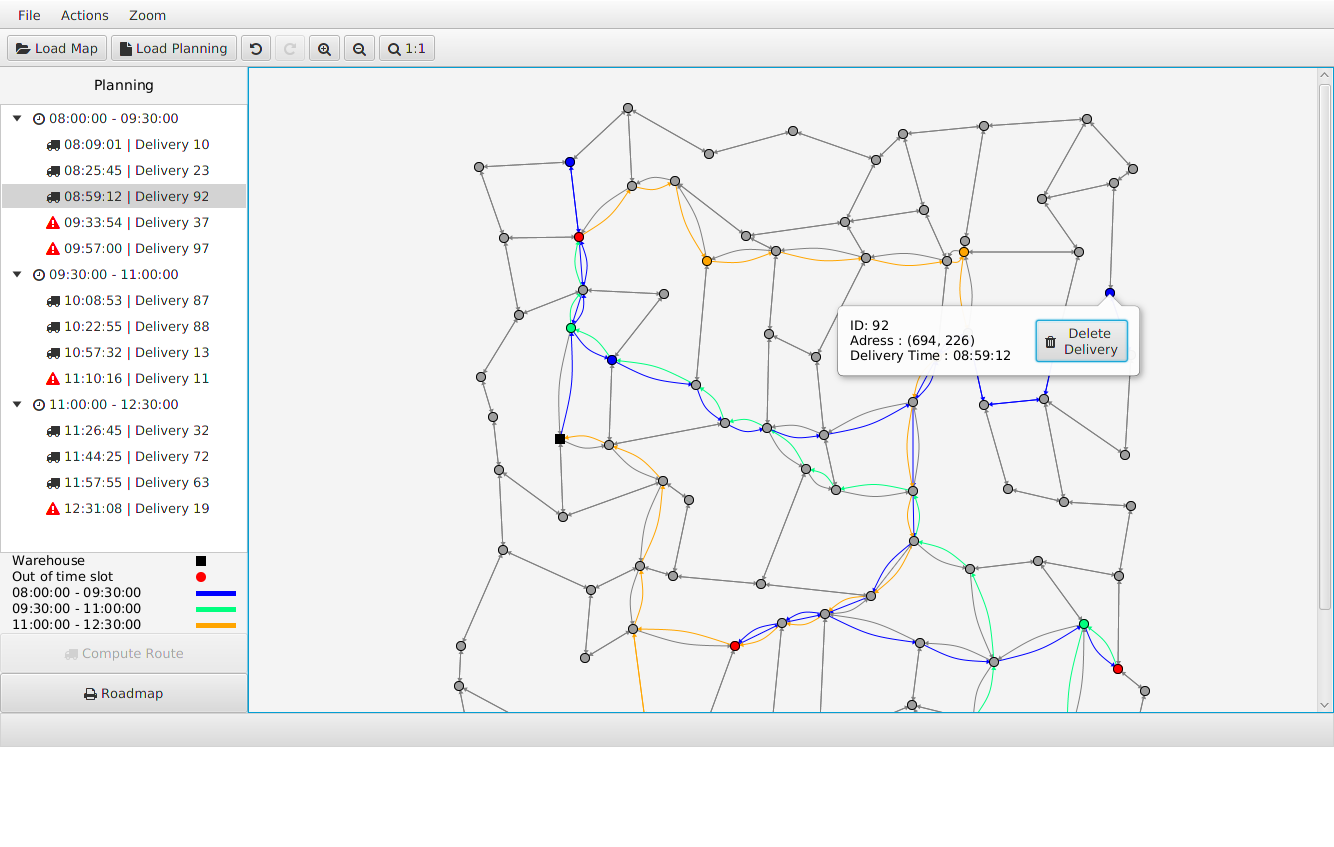
\includegraphics[width=\textwidth]{figures/screenshot.png}}
\noindent\makebox[\textwidth]{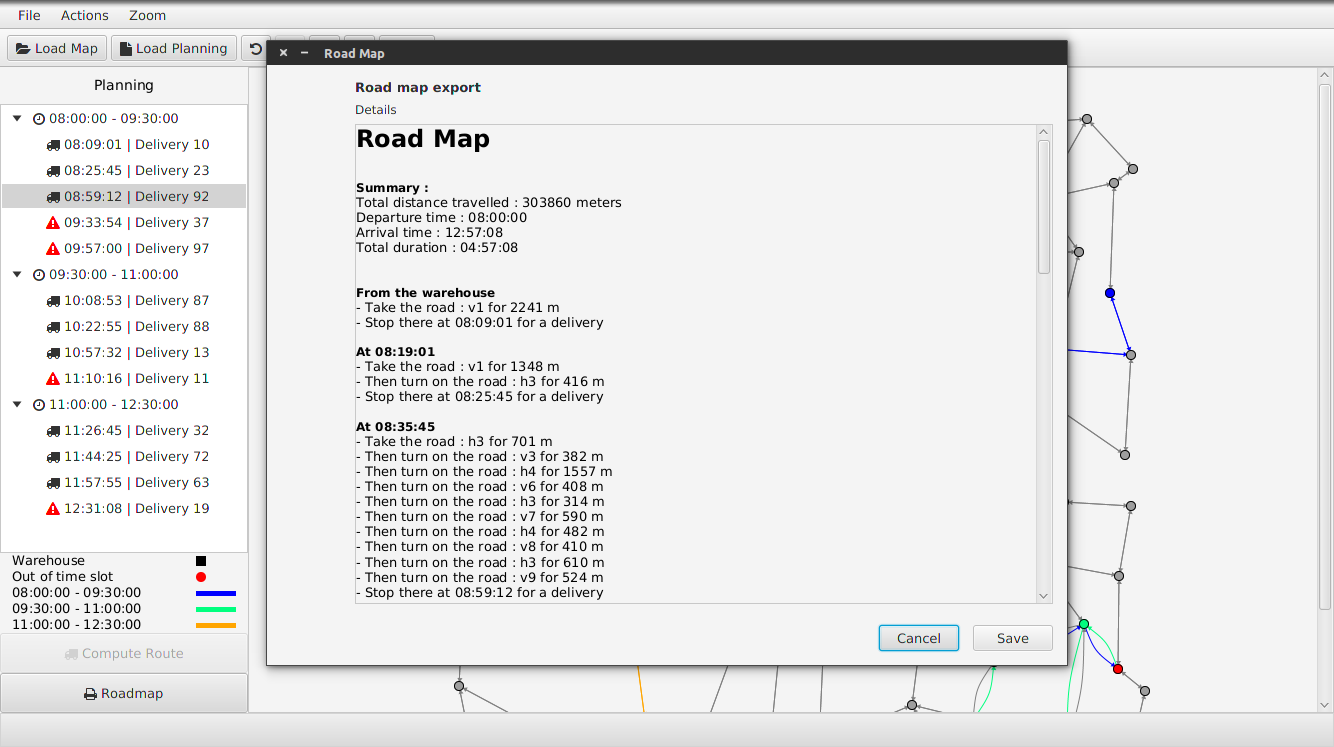
\includegraphics[width=\textwidth]{figures/screenshot-1.png}}
\caption{Captures d'écran du logiciel}
\end{figure}




%%%%%%%%%%%%%%%%%%%%%%%%%%%%%%%%%%%%%%%%% Capture et analyse des besoins

\part{Capture et analyse des besoins}
\label{part:capture-et-analyse-des-besoins}
\setcounter{section}{0}

\section{Planning prévisionnel du projet \it{(FR)}}
\label{sec:planning-previsionnel-du-projet}

Voici le diagramme de Gantt du déroulement du projet.
Nous avions estimé que le projet devait être bien avancé pendant les vacances de la semaine 44 et finaliser les détails durant la semaine 45 ne sachant pas la date initiale du rendu. Bien entendu nous avons étendu la phase d'implémentation une fois cet élément manquant acquis (cf. diagramme de Gantt réel~\ref{sec:planning-effectif-du-projet}).

\begin{figure}[H]
\centering
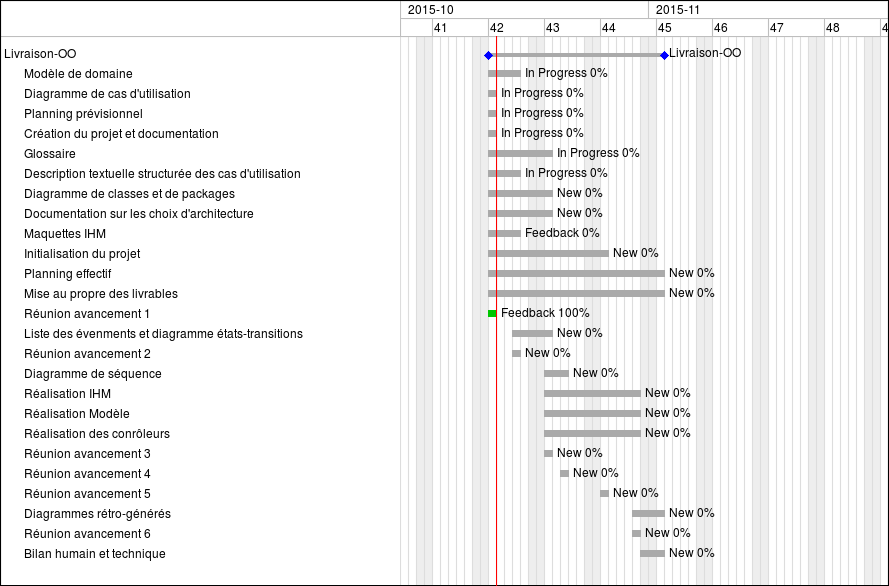
\includegraphics[scale=0.5,angle=0]{redmine/gantt-prev.png}
\caption{Planning prévisionnel}
\end{figure}

Voici la répartition globale des tâches ainsi qu'une rapide estimation des temps pour chacune d'elles afin d'avoir un retour plus conséquent en fin de projet sur le planning prévisionnel.

\begin{figure}[H]
\begin{center}
\begin{tabular}{  l  l  l  }
  \hline
  \bf{Tâche} & \bf{Affectation} & \bf{Temps estimé} \\
  \hline
  %%%% Gestion de projet
  \hline
  \bfit{Gestion de projet} & \multicolumn{2}{r}{\it{Sous-Total : 41 heures}} \\
  \hline
  Création du projet et documentation & Hugues & 3 heures \\
  \hline
  Initialisation du projet & Tous & 2 heures \\
  \hline
  Réunion d'avancement 1 & Antoine & 3,5 heures \\
  \hline
  Réunion d'avancement 2 & Antoine & 3,5 heures \\
  \hline
  Réunion d'avancement 3 & Antoine & 3,5 heures \\
  \hline
  Réunion d'avancement 4 & Antoine & 3,5 heures \\
  \hline
  Réunion d'avancement 5 & Antoine & 3,5 heures \\
  \hline
  Réunion d'avancement 6 & Antoine & 3,5 heures \\
  \hline
  Finalisation des livrables & Tous & 15 heures \\
  \hline
  %%%% Analyse des besoins
  \hline
  \bfit{Analyse des besoins} & \multicolumn{2}{r}{\it{Sous-Total : 18,5 heures}} \\
  \hline
  Modèle de domaine & Estelle, Lisa et Paul & 9 heures \\
  \hline
  Diagramme de cas d'utilisation & Guillaume, Pierre & 2 heures \\
  \hline
  Planning prévisionnel & Antoine & 2 heures \\
  \hline
  Glossaire & Paul, Estelle, Lisa & 1,5 heure \\
  \hline
  Description textuelle structurée des cas d'utilisation & Pierre, Guillaume & 4 heures \\
  \hline
  %%%% Conception
  \hline
  \bfit{Conception} & \multicolumn{2}{r}{\it{Sous-Total : 25 heures}} \\
  \hline
  Liste des évenments et diagramme états-transitions & Estelle, Guillaume et Antoine & 6 heures \\
  \hline
  Diagramme de classes et de packages & Pierre, Paul, Hugues & 12 heures \\
  \hline
  Documentation choix architecture & Paul, Hugues & 3 heures \\
  \hline
  Maquettes IHM & Lisa et Hugues & 2 heures \\
  \hline
  Diagramme de séquence & Pierre & 2 heures \\
  \hline
  %%%% Implémentation et tests
  \hline
  \bfit{Implémentation et tests} & \multicolumn{2}{r}{\it{Sous-Total : 52 heures}} \\
  \hline
  Réalisation IHM & Hugues & 20 heures \\
  \hline
  Réalisation Modèle & Pierre, Lisa et Guillaume & 15 heures \\
  \hline
  Réalisation des contrôleurs & Estelle, Paul et Antoine & 15 heures \\
  \hline
  Diagramme rétro-générés & Antoine & 2 heures \\
  \hline
  %%%% Bilan
  \hline
  \bfit{Bilan} & \multicolumn{2}{r}{\it{Sous-Total : 6 heures}} \\
  \hline
  Planning effectif & Antoine & 2 heures \\
  \hline
  Bilan humain et technique & Antoine & 4 heures \\
  \hline
  %%%% Total
  \hline
  \multicolumn{3}{r}{\bf{Total temps estimé :} 142,5 heures} \\
  \hline
\end{tabular}
\end{center}
\caption{Affectations et estimations des tâches}
\end{figure}

Un certain nombre de tâches supplémentaires sont arrivés ensuite ainsi qu'un redécoupage en sous-tâches pour l'implémentation. Le temps estimé a donc été augmenté une fois que nous avions une vision plus complète sur le travail à effectuer (analyse des besoins et conception terminées).

\section{Domain model \it{(EN)}}
\label{sec:domain-model}

This application has two main entry points that are the Map and Planning classes. The first one is used to represent the streets (directed arcs) and intersections (nodes) of a city, using a graph design. The class Planning represents the set of deliveries that must be done at some locations, in particular time slots. Those data are represented through the TimeSlot and Delivery classes.\\

The Route class represents the best known solution to do all the delivery points contained in the Planning object, thanks to an ordered collection of Path. A Path is itself an ordered collection of arcs to use to go from a node with a delivery (or a warehouse) to another node with a delivery (or a warehouse).\\

The delivery time attribute in the Delivery class is rather important because it's the time that is affected to a delivery when a route is computed.

\begin{figure}[H]
\centering
\noindent\makebox[\textwidth]{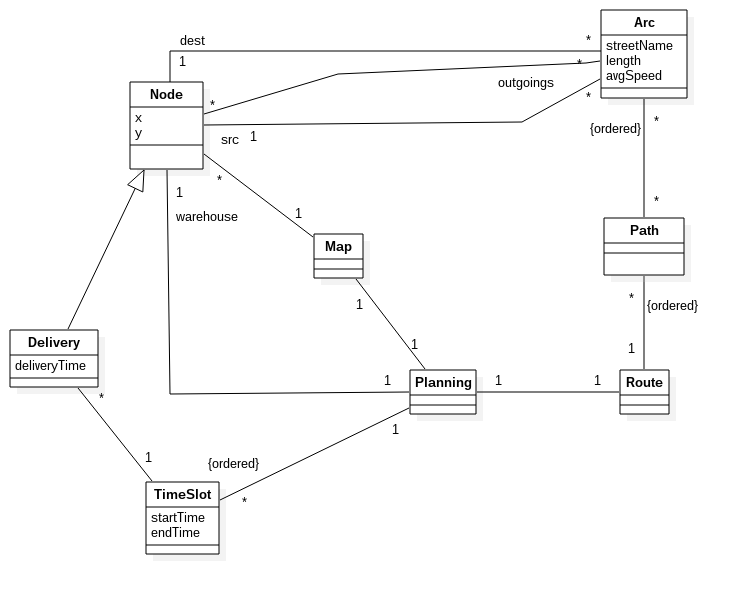
\includegraphics[width=\textwidth]{figures/domain-model.png}}
\caption{Domain Model}
\end{figure}

\section{Glossary \it{(EN)}}
\label{sec:glossary}

Syntax used :
\begin{itemize}
	\item[\textbullet] \bf{Object} \it{(french equivalent)} : definition \\
\end{itemize}

Glossary : 
\begin{itemize}
	\item[\textbullet] \bf{Arc} \it{(tronçon)} : section of road between two intersections described by a street name, an average speed, a length and the id of the destination intersection.
	\item[\textbullet] \bf{Node} \it{(intersection)} : Intersection between two or more arcs (cf. Arc) described by its coordinates and an id.
	\item[\textbullet] \bf{Path} \it{(chemin)} : Ordered list of arcs between two delivery nodes, representing the shortest travel duration.
	\item[\textbullet] \bf{Map} \it{(plan)} : Set of arcs (cf. Arc) and intersections (cf. Node)
	\item[\textbullet] \bf{Delivery} \it{(livraison)} : Special node which must be contained by the final route.
	\item[\textbullet] \bf{Planning} : Set of intersections (cf. Node) to be processed by the route computation algorithm (cf. Route).
	\item[\textbullet] \bf{Route} \it{(tournée)} : Ordered list of paths to travel along (cf. Planning). 
	\item[\textbullet] \bf{TimeSlot} \it{(fenêtre de livraison)} : time interval bounded by a start time and an end time containing a set of deliveries to be honored.
	\item[\textbullet] \bf{Warehouse} \it{(entrepôt)} : Special intersection representing both the start and the end point of the route (cf. Route).
	\item[\textbullet] \bf{Average Speed} \it{(vitesse moyenne)} : average speed of vehicles in meters per second on an arc (cf. Arc).
	\item[\textbullet] \bf{Planning File} \it{(fichier de planning)} : XML formated input file, describing a planning (cf. Planning).
	\item[\textbullet] \bf{Map File} \it{(fichier de plan)} : XML formated input file, describing a Map.
	\item[\textbullet] \bf{Route File} \it{(fichier d’itinéraire)} : text formated output file, describing paths to travel along.
\end{itemize}

\section{Use case diagram \it{(EN)}}
\label{sec:use-case-diagram}

This application doesn’t have any user access control, so only the user role can be represented as a main actor, in the following use cases diagram. However, we can see a second actor, called \og Files system \fg{}, related to the use cases \og Load Map \fg{}, \og Load Planning \fg{} and \og Export Route \fg{}. Those use cases require at least one reading or writing file interaction, managed by the \og Files system \fg{} actor, mostly managed itself by the operating system.\\

The use case \og Edit Route \fg{} could be split in three sub-parts - \og Add a delivery \fg{}, \og Remove a delivery \fg{} and \og Swap two deliveries \fg{} - but we choose to keep only one use case. Indeed, if the application will be improved with several new edit route features, it won’t be necessary to update the diagram with too many use cases.\\

Each use case is detailed further in the following section, through the textual descriptions.

\begin{figure}[H]
\centering
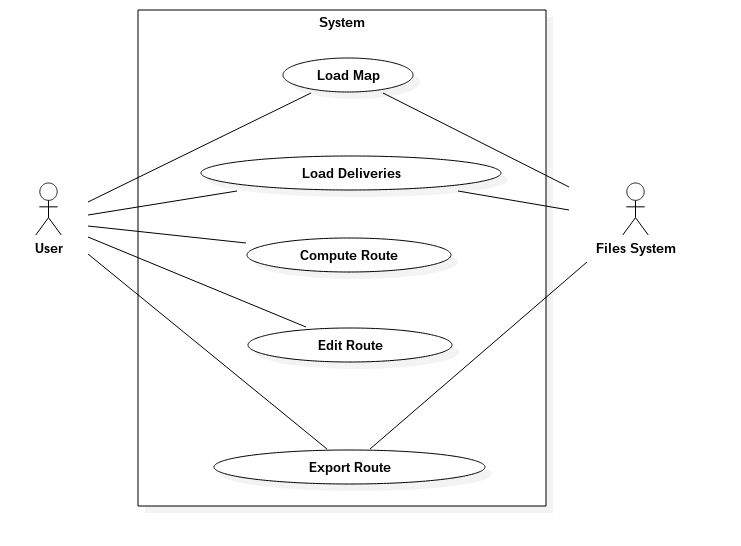
\includegraphics[scale=0.5,angle=0]{figures/use-case.png}
\caption{Use case diagram}
\end{figure}

\section{Structured textual description of use cases \it{(EN)}}
\label{sec:structured-textual-description-of-use-cases}

\subsection{Textual description of \it{Load map}}
\label{subsec:textual-description-of-load-map}

\textbf{Short description :} The user selects an XML file describing a city map. The map is loaded and displayed on the screen.

\textbf{Organized description :}

\begin{itemize}
  \item[•] \textbf{Precondition :} none.
  \item[•] \textbf{Main scenario :}
  \begin{enumerate}
    \item The user indicates that he wants to load a map
    \item The system opens a dialog box allowing the user to select a file.
    \item The user selects the XML file describing the map that he wants to load in the program.
    \item The system interprets the XML file, loads the city map and display the map on the screen.
    \item The user can’t cancel his former modifications anymore.
  \end{enumerate}
  \item[•] \textbf{Alternative scenarios :}
  \begin{itemize}
    \item[3.] The users indicates that he wants to stop the selection of a city map.
    \begin{itemize}
      \item[•] Le system stops the selection and ends the scenario.
    \end{itemize}
    \item[4a.] The XML file selected is incorrect (cf. XML Errors Lists~\ref{subsec:xml-errors-lists}) and doesn’t define a city map.
    \begin{itemize}
      \item[•] The system indicates that the file is incorrect and can’t be loaded, and end the scenario.
    \end{itemize}
    \item[4b.] The opening and the reading of the XML file is denied (cf. IO Errors Lists~\ref{subsec:io-errors-list}).
    \begin{itemize}
      \item[•] The system displays that the loading has failed and indicates the cause (insufficient privileges…) and ends the scenario.
    \end{itemize}
  \end{itemize}
\end{itemize}

\subsection{Textual description of \it{Load delivery request}}
\label{subsec:textual-description-of-load-delivery-request}

\textbf{Short description :} The user selects an XML file describing delivery requests. The system displays the position of each delivery request on the city map.

\textbf{Organized description :}

\begin{itemize}
  \item[•] \textbf{Precondition :} a city map has to be loaded.
  \item[•] \textbf{Main scenario :}
  \begin{enumerate}
    \item The user indicates that he wants to load a delivery request.
    \item The system asks the user to select an XML file in the file system.
    \item The user selects an XML file.
    \item The system interprets the XML file and loads delivery requests, then it deletes the modifications history and displays the delivery points on the city map.
  \end{enumerate}
  \item[•] \textbf{Alternative scenarios :}
  \begin{itemize}
    \item[3.] The user indicates that he wants to stop the selection of the delivery requests.
    \begin{itemize}
      \item[•] The system stops the selection and ends the scenario.
    \end{itemize}
    \item[4a.] The XML file selected is incorrect (cf. XML Errors list~\ref{subsec:xml-errors-lists}) and doesn’t define delivery requests.
    \begin{itemize}
      \item[•] The system indicates that the file is incorrect and can’t be loaded, then it ends the scenario.
    \end{itemize}
    \item[4b.] The opening and the reading of the XML file is denied (cf. IO Errors Lists~\ref{subsec:io-errors-list}).
    \begin{itemize}
      \item[•] The system displays that the generation has failed and indicates the cause (insufficient privileges…) and ends the scenario.
    \end{itemize}
  \end{itemize}
\end{itemize}

\subsection{Textual description of \it{Compute a route}}
\label{subsec:textual-description-of-compute-a-route}

\textbf{Short description :} The users asks the system to compute a route. The route computed by the system is displayed on the screen, as the list of deliveries.

\textbf{Organized description :}

\begin{itemize}
  \item[•] \textbf{Precondition :} a file of delivery requests has to be loaded.
  \item[•] \textbf{Main scenario :}
  \begin{enumerate}
    \item The users asks the system to compute the route.
    \item The system computes the path of the route and displays it on the city map, indicating deliveries that will be late (out of the planned time slot). The system also displays the list of deliveries, in the order of the route, with the time slot and the hour estimated of each delivery.
  \end{enumerate}
  \item[•] \textbf{Alternative scenarios :}
  \begin{itemize}
    \item[1-2.] The user indicates to the system that he wants to interrupt the computing of the route.
    \begin{itemize}
      \item[•] The systems interrupts the computing and ends the scenario.
    \end{itemize}
  \end{itemize}
\end{itemize}

\subsection{Textual description of \it{Add a delivery}}
\label{subsec:textual-description-of-add-a-delivery}

\textbf{Short description :} The user adds a delivery to the route, at a node that isn’t already a delivery point.

\textbf{Organized description :}

\begin{itemize}
  \item[•] \textbf{Precondition :} a route has to be computed.
  \item[•] \textbf{Main scenario :}
  \begin{enumerate}
    \item The user indicates that he wants to add a delivery to the route.
    \item The system asks the user to select an empty node, where the delivery will be added.
    \item The user selects the node where the delivery will be executed.
    \item The system asks the user to select the delivery that will be executed before the one he wants to add.
    \item The user selects the delivery that will be executed before the one he wants to add.
    \item The system selects a default time slot (the same time slot as the one of the delivery that will be executed before the new one).
    \item The user confirms the new delivery request.
    \item The system adds the new delivery, updates the path between the previous point and the next point and refreshes the displaying of the map and the route. The delivery times are also reloaded.
  \end{enumerate}
  \item[•] \textbf{Alternative scenarios :}
  \begin{itemize}
    \item[2.] The user selects a node that is already a delivery point.
    \begin{itemize}
      \item[•] The system displays an error message and ends the scenario.
    \end{itemize}
    \item[6.] The user selects another time slot than the one which is selected by default, in the list of the time slots that already exists.
    \begin{itemize}
      \item[•] The system takes the time slot chosen by the user and goes to the step 7.
    \end{itemize}
    \item[1-7.] The user interrupts his request.
    \begin{itemize}
      \item[•] The request isn’t taken into account and the system ends the scenario.
    \end{itemize}
  \end{itemize}
\end{itemize}

\subsection{Textual description of \it{Delete a delivery}}
\label{subsec:textual-description-of-delete-a-delivery}

\textbf{Short description :} The user deletes an existing delivery of the route.

\textbf{Organized description :}

\begin{itemize}
  \item[•] \textbf{Precondition :} a route has to be computed.
  \item[•] \textbf{Main scenario :}
  \begin{enumerate}
    \item The user selects a delivery and indicates that he wants to delete it.
    \item The system shows a deletion confirmation.
    \item The user confirms the deletion.
    \item The system deletes the delivery, updates the path between the previous delivery and the next one and displays the new route.
  \end{enumerate}
  \item[•] \textbf{Alternative scenarios :}
  \begin{itemize}
    \item[3.] The user cancels his deletion request.
    \begin{itemize}
      \item[•] The deletion request isn’t taken into account and the system ends the scenario.
    \end{itemize}
  \end{itemize}
\end{itemize}

\subsection{Textual description of \it{Swap two deliveries}}
\label{subsec:textual-description-of-swap-two-deliveries}

\textbf{Short description :} The user swaps two deliveries.

\textbf{Organized description :}

\begin{itemize}
  \item[•] \textbf{Precondition :} a route has to be computed.
  \item[•] \textbf{Main scenario :}
  \begin{enumerate}
    \item The user moves graphically the delivery on another delivery. If the delivery time of the selected delivery is lower (respectively higher) than the delivery time of the second one, then the second delivery has to be executed before (respectively after) the first one.
    \item The system updates the path of the route and displays it.
  \end{enumerate}
  \item[•] \textbf{Alternative scenarios :}
  \begin{itemize}
    \item[1-2.] The user interrupts his swap request.
    \begin{itemize}
      \item[•] The swap request isn’t taken into account and the system ends the scenario.
    \end{itemize}
    \item[2a.]  The user drop the delivery to move on the same node where it was before, or on an area that isn’t a delivery node.
    \begin{itemize}
      \item[•] The system ignores the swap and ends the scenario.
    \end{itemize}
  \end{itemize}
\end{itemize}

\subsection{Textual description of \it{Generate an itinerary}}
\label{subsec:textual-description-of-generate-an-itinerary}

\textbf{Short description :} The user asks the system to generate an itinerary.

\textbf{Organized description :}

\begin{itemize}
  \item[•] \textbf{Precondition :} a route has to be computed.
  \item[•] \textbf{Main scenario :}
  \begin{enumerate}
    \item The user indicates that he wants to generate an itinerary.
    \item The system asks the user to name the file and to select the location where it will be saved.
    \item The user names the file and selects a location.
    \item The system generates an itinerary in txt format, with the list of the deliveries, and displays a message on the screen when it’s done.
  \end{enumerate}
  \item[•] \textbf{Alternative scenarios :}
  \begin{itemize}
    \item[3.] The user indicates that he wants to interrupt the generation.
    \begin{itemize}
      \item[•] The system stops the generation and ends the scenario.
    \end{itemize}
    \item[4.]  The record is denied.
    \begin{itemize}
      \item[•] The system displays that the generation failed and indicates the cause (insufficient privileges…) and ends the scenario.
    \end{itemize}
  \end{itemize}
\end{itemize}

\subsection{Alternative scenarios that can occur at any moment}
\label{subsec:alternative-scenarios-that-can-occur-at-any-moment}

\begin{itemize}
  \item[a.] The user chooses to cancel his last modification.
  \begin{itemize}
    \item[•] The system cancels the last modification if it exists and restores the previous route.
  \end{itemize}
  \item[b.] The users chooses to redo a cancelled modification.
  \begin{itemize}
    \item[•] The system redoes the last cancelled modification if it exists, and restores the corresponding route.
  \end{itemize}
\end{itemize}

%%%%%%%%%%%%%%%%%%%%%%%%%%%%%%%%%%%%%%%%%%%%%%%%%%%%%%%%%%%% Conception
\part{Conception}
\label{part:conception}
\setcounter{section}{0}

\section{User-level events list and State-Transition Diagram \it{(EN)}}
\label{sec:user-level-events-list-and-state-transition-diagram}

\bf{State-transition diagram:}
At any moment, the user can exit the program.
At the opening, the program is in InitState. Right there, the only thing he can do is selecting a map (MapSelectState). From this state, he can either select a map (from an XML file) and go to MapLoadedState, or go back to InitState. If he decides to select a map, then the same process repeats with the selection of a planning (PlanningSelectState). Then he either comes back to MapLoadedState and pick a planning and ends in PlanningLoadedState. From this point, he has many options:\\

\begin{itemize}
  \item[•] Select a new planning (PlanningSelectState).
  \item[•] Select a new map (MapSelectState).
  \item[•] Go back to the beginning (InitState)
  \item[•] Compute the route (ComputingRouteState).\\
\end{itemize}

If he decides to compute the route and everything is fine, the program will be in NothingSelectedState, where you just have the map with the route computed but you don't have any node selected on the mpa or on the tree list. Here, the user has two choices:\\

\begin{itemize}
  \item[•] Clicking on an existing delivery (going to DeliverySelectedState).
  \item[•] Clicking on an emptyNode (goingto EmptyNodeSelected).\\
\end{itemize}

From the first choice, the user can go to the second one, and from the second one he can go to the first one. If he is in DeliverySelectedState and he decides to remove the delivery by clicking the remove-button, he goes to EmptyNodeSelected.
From both choices, it is also possible to click on the warehouse (going to WarehouseSelectedState), and to comeback to NothingSelectedState by clicking anywhere else on the map.
After computing the route, at any moment the user can:\\

\begin{itemize}
  \item[•] Swap two deliveries (SwapDeliveriesState): it's something a bit different here, because we use the drag and drop. To access to this state, the user has to left click a delivery and keep it pressed. To leave this state, he has to release the left click, either on a delivery (so the two deliveries will be swapped) or not on a delivery (so nothing happens). In both cases, the program comes back to NothingSelectedState.
  \item[•] Undo his last action.
  \item[•] Redo the last cancelled action.
  \item[•] Go back to PlanningSelectState by clicking "Load Planning" or "Clear History".
  \item[•] Go back to MapLoadedState by clicking "Clear Planning" or "Clear History".
  \item[•] Go back to MapSelectState by clicking "Load Map" or "Clear History".
  \item[•] Go back to InitState by clicking "Close Map" or "Clear History".\\
\end{itemize}

\bf{The user-level events list :}
\begin{itemize}
  \item[•] \it{btnLoadMap :} the user request to load a new map from a XML file.
  \item[•] \it{btnLoadPlanning :} the user request to load a new planning from a XML file.
  \item[•] \it{btnGenerateRoute :} the event to compute the fastest route to make all deliveries.
  \item[•] \it{btnCancel :} the user request to cancel the current process.
  \item[•] \it{btnValidateFile :} the user request to validate a file selected.
  \item[•] \it{leftClickPressedOnDelivery :} when the user make a left click pressed on a delivery.
  \item[•] \it{leftClickReleased :} when the user releaded the previous left click pressed on a delivery.
  \item[•] \it{clickOnDelivery :} when the user make a simple click on a delivery.
  \item[•] \it{clickSomewhereElse :} when the user click on something not interactive in the application.
  \item[•] \it{clickOnEmptyNode :} when the user mae a simple click on an empty node.
  \item[•] \it{btnAddDelivery :} the user request to add a new delivery on a previous empty node selected.
  \item[•] \it{btnRemoveDelivery :} the user request to remove a delivery previously selected.
  \item[•] \it{clickOnWarehouse :} when the user make a simple click on the warehouse.
  \item[•] \it{btnCloseMap :} the user request to close the current map loaded.
  \item[•] \it{btnClearPlanning :} the user request to close the current planning loaded.
\end{itemize}

\begin{figure}[H]
\noindent\makebox[\textwidth]{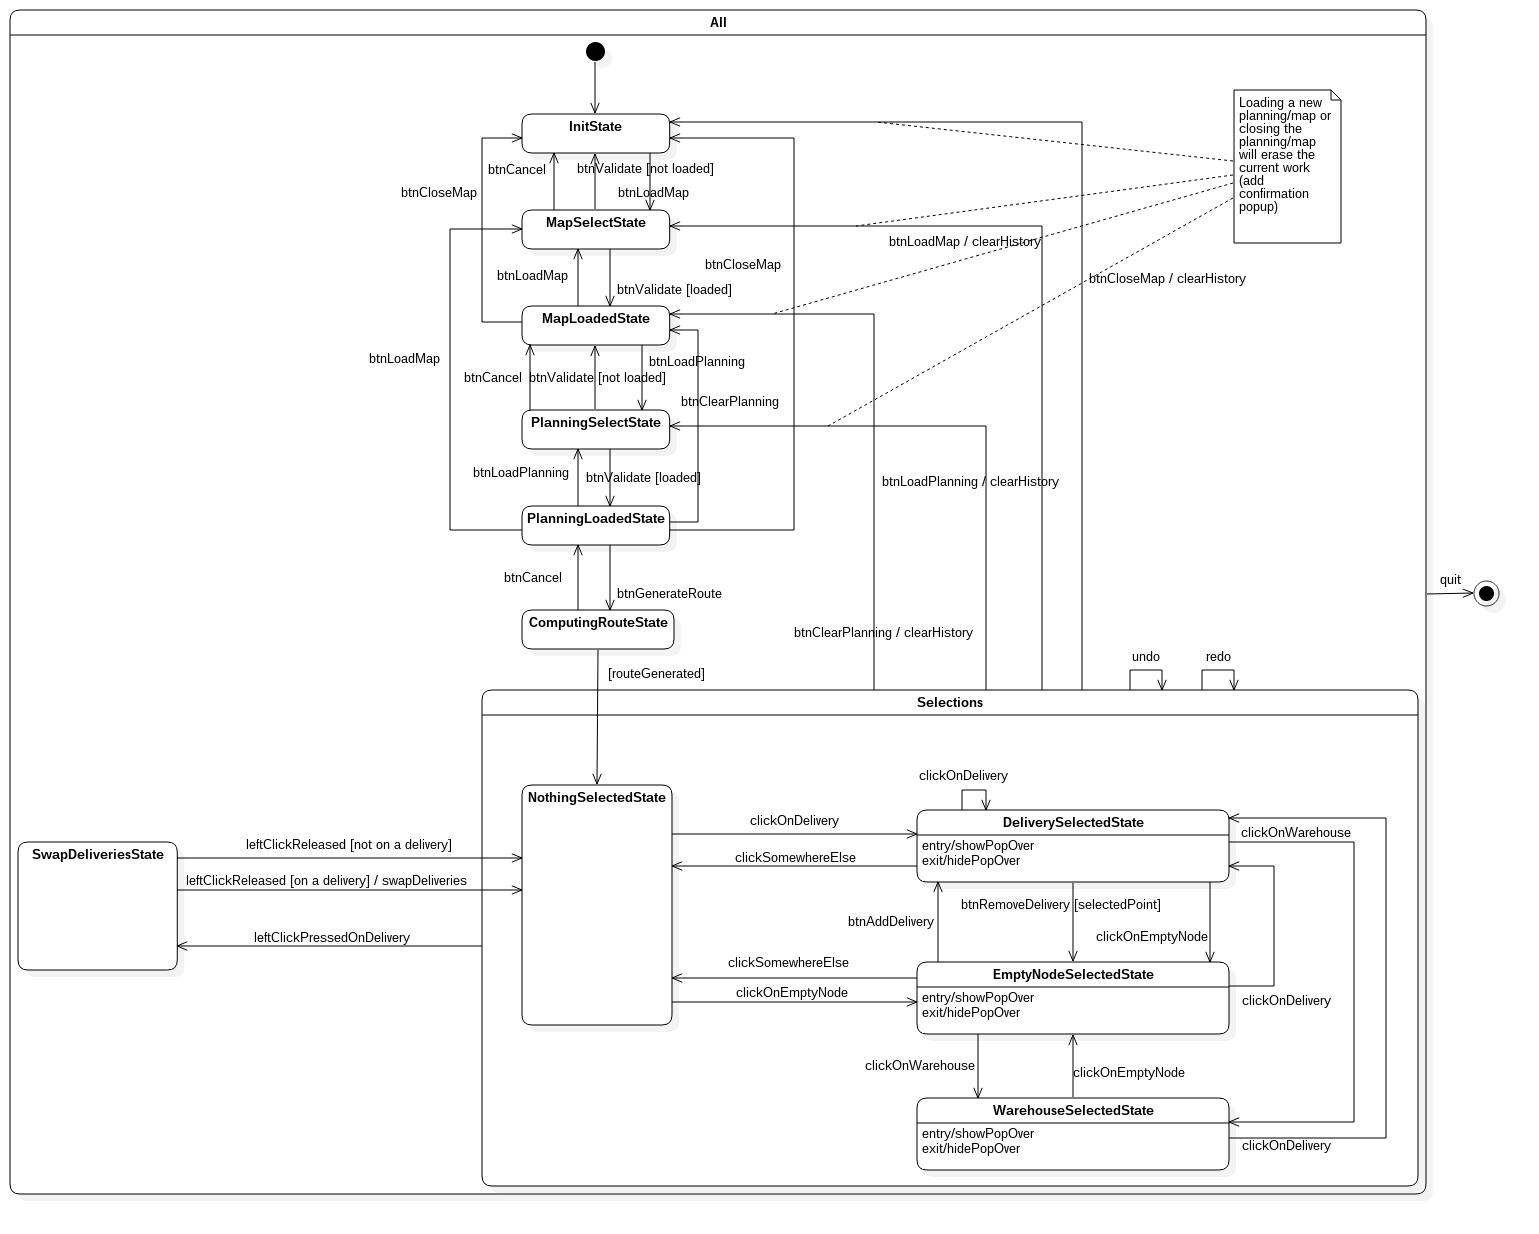
\includegraphics[scale=0.43,angle=90]{figures/state-machine.png}}
\caption{State-Transition Diagram}
\end{figure}

\newpage

\section{Packages and Classes Diagrams \it{(EN)}}
\label{sec:packages-and-classes-diagrams}

\subsection{Model related diagrams}
\label{subsec:model-related-diagrams}

The following figure shows classes which are part of the model package. These classes implements the Domain Model and others objects needed to properly use design patterns. All methods are not shown, especially getters and setters. Further information are available in III.3 section.\\

\begin{center}
\vspace*{-6cm}
\begin{figure}[H]
\centering
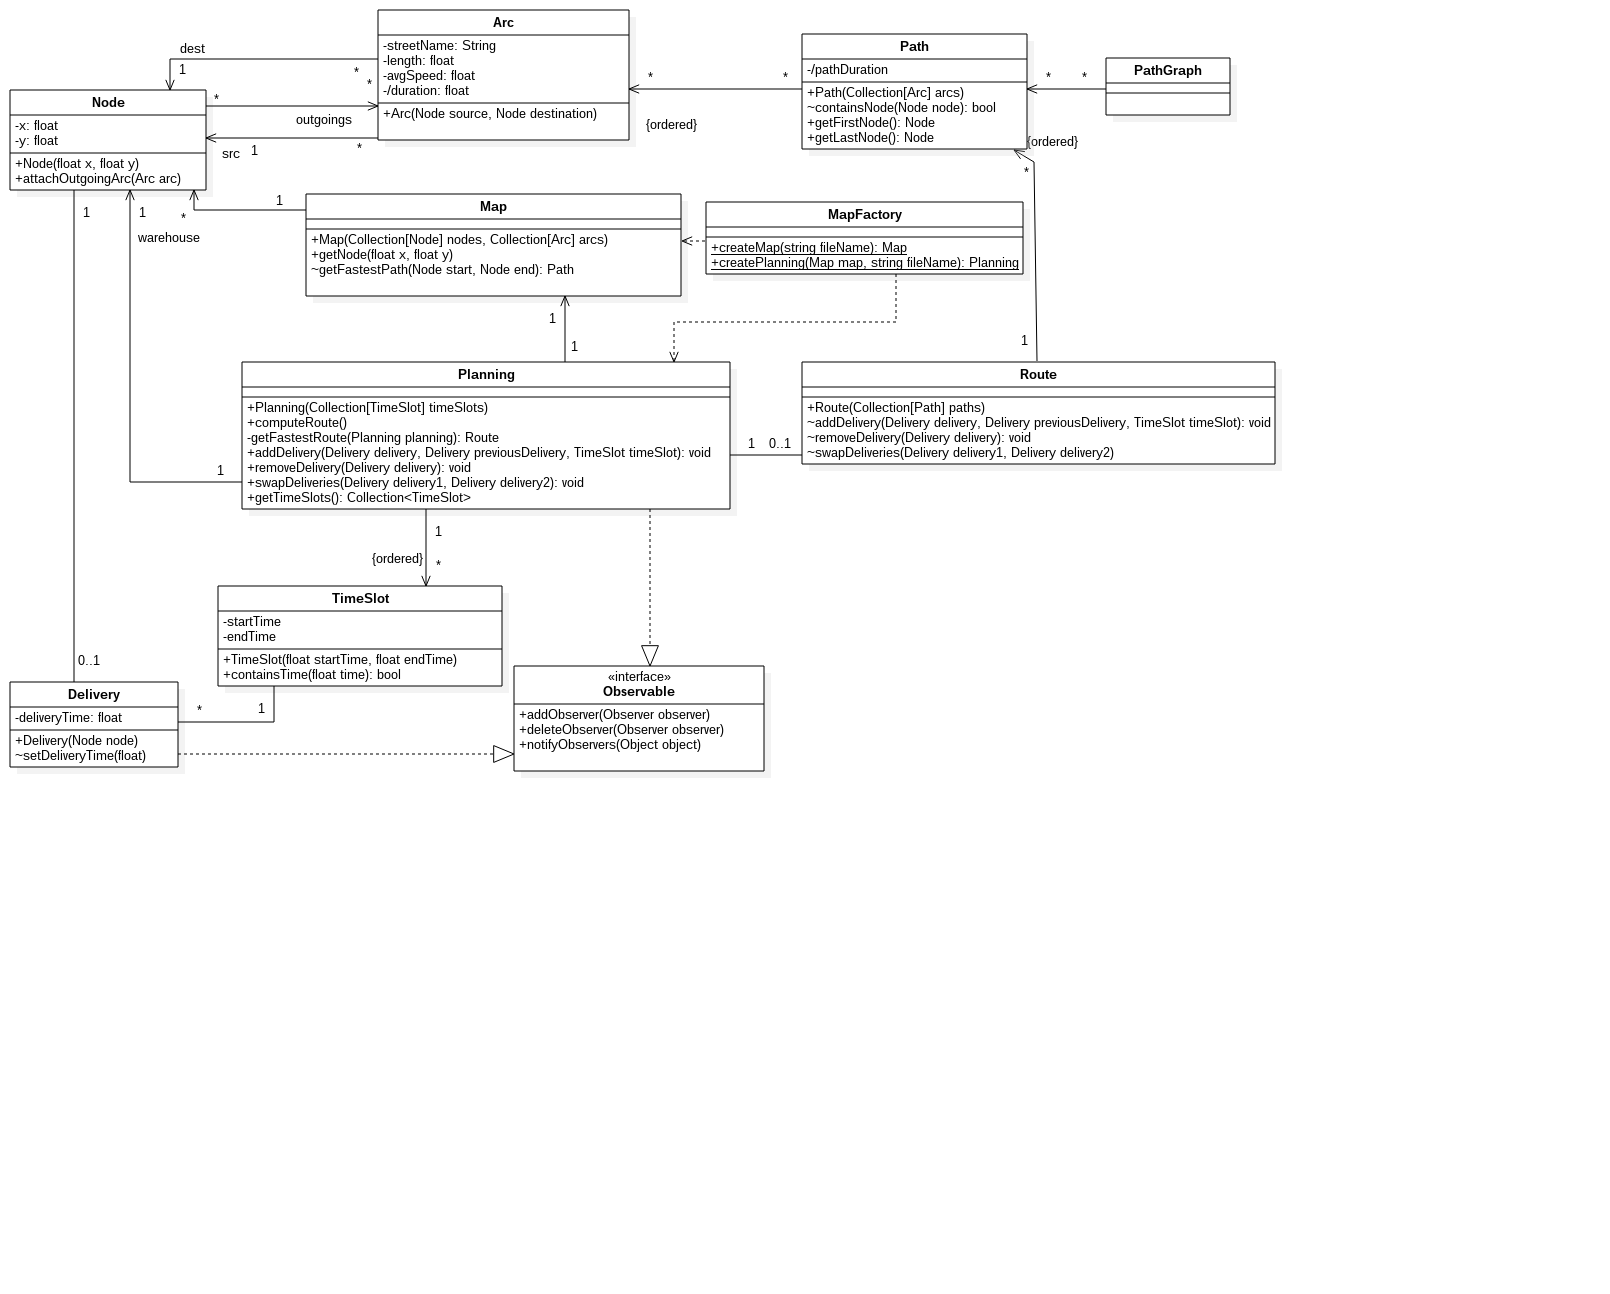
\includegraphics[scale=0.47,angle=90]{figures/model-class.png}
\caption{Model package including classes}
\end{figure}
\end{center}

\subsection{View related diagrams}
\label{subsec:view-related-diagrams}

The following figure presents the view package, it is reduced to objects linked directly or indirectly to the Domain Model. Some objects such as PopOverContent and its derivates exists due to technological choices made to represent information about nodes and the way user will interact with them. UIManager which is part of the controller package but is strongly related to this package as it is in charge of instanciating the MainWindow. Further information are available in III.3 section.

\begin{figure}[H]
\noindent\makebox[\textwidth]{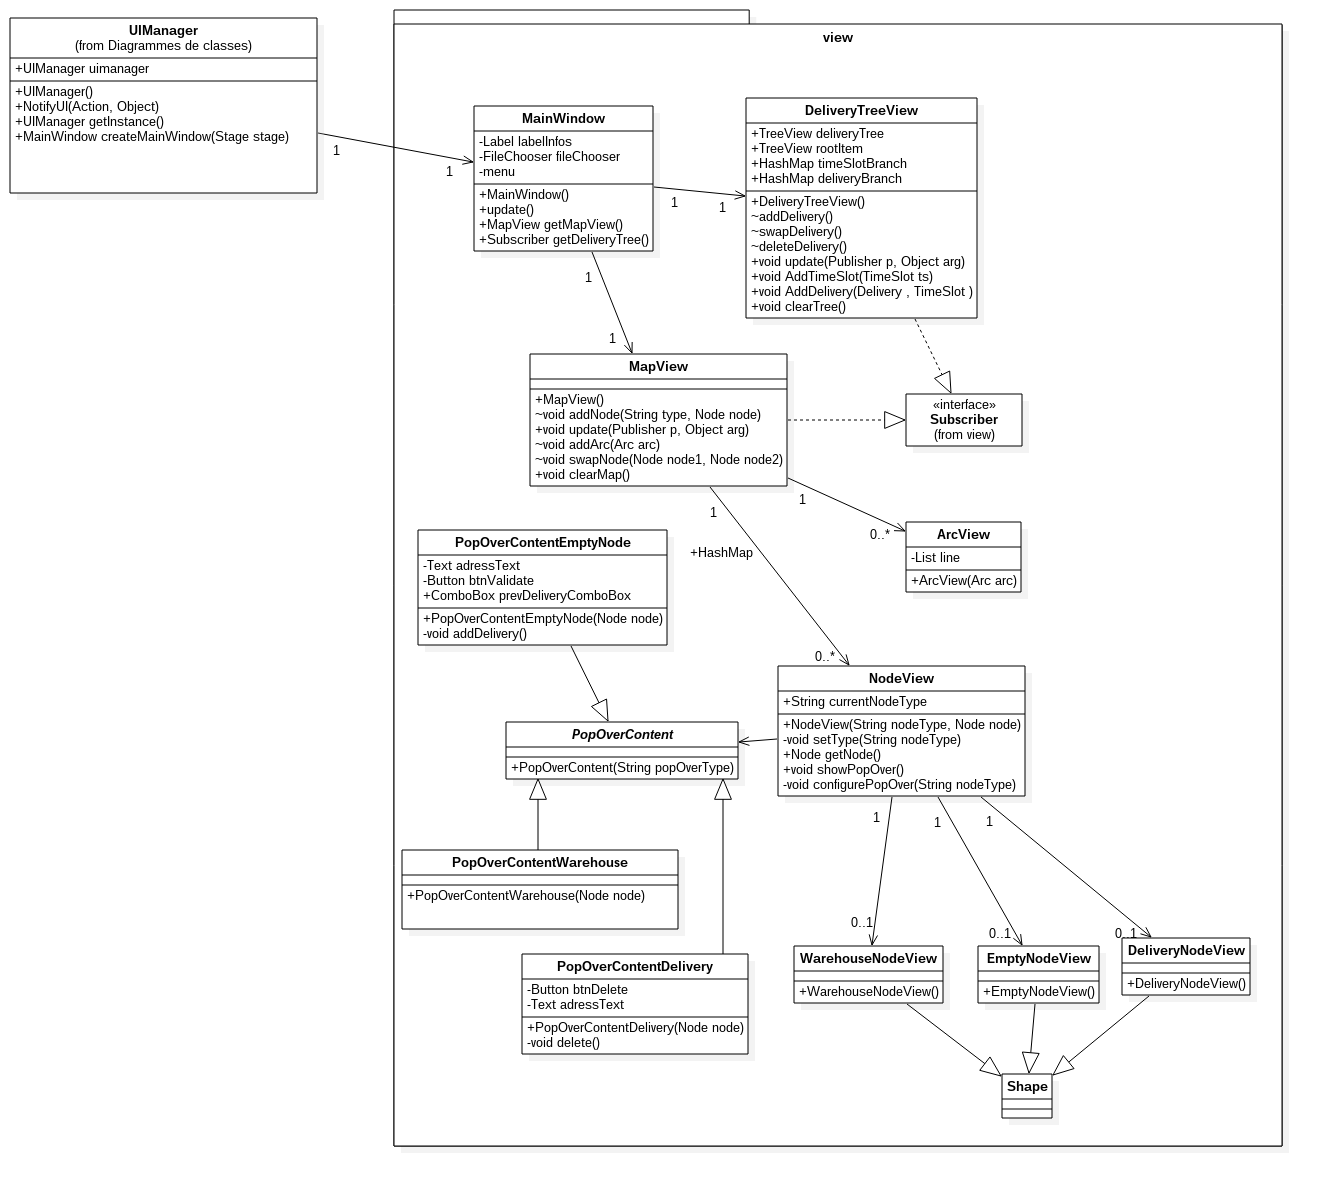
\includegraphics[scale=0.40,angle=0]{figures/view-class.png}}
\caption{View package including classes}
\end{figure}

\subsection{Controller related diagrams}
\label{subsec:controller-related-diagrams}

The three following figures show how we designed the controller. The controller is in fact divided into four Managers which are in reality sub-controllers dedicted to specific tasks. They have been named according to their role. Two more packages, states and commands, have been added to implement State and Command design patterns. These two packages are used by the ContextManager which is charged of assuring application process consistency. Further information are available in III.3 section.  

\begin{figure}[H]
\centering
\noindent\makebox[\textwidth]{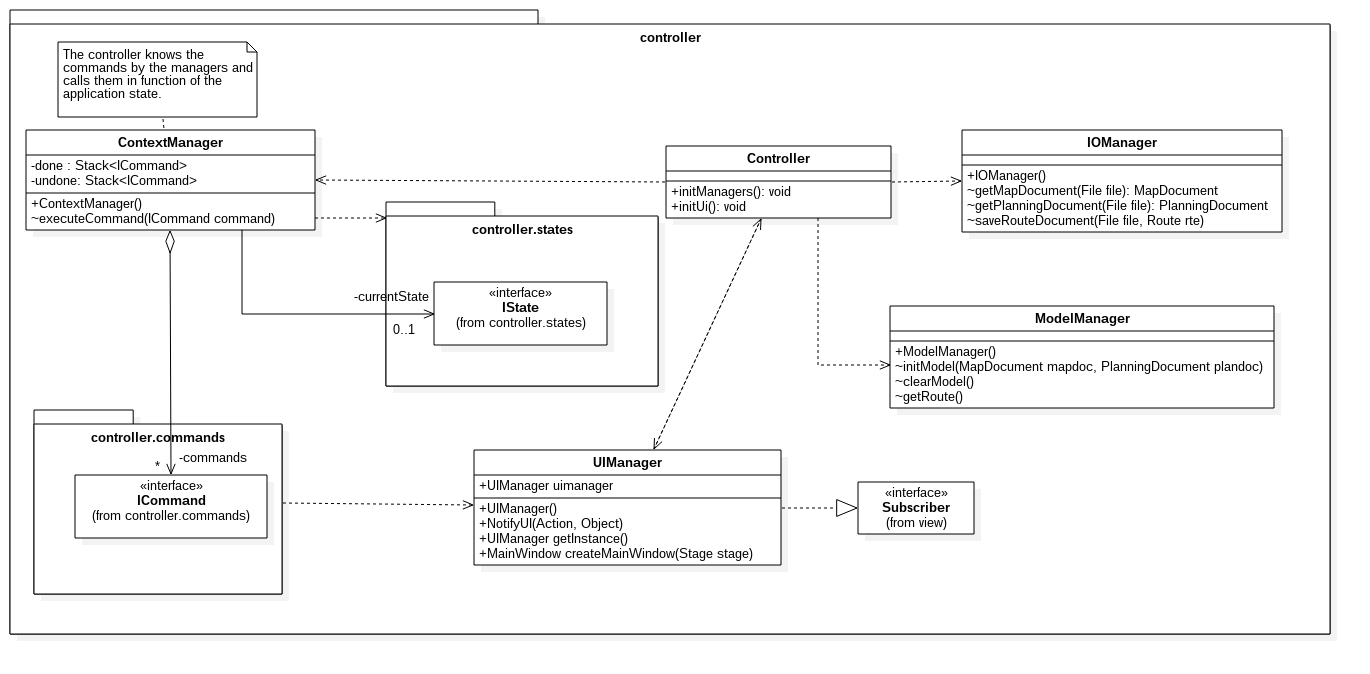
\includegraphics[scale=0.5,angle=90]{figures/controller-class.png}}
\caption{Controller package including classes}
\end{figure}

\begin{figure}[H]
\noindent\makebox[\textwidth]{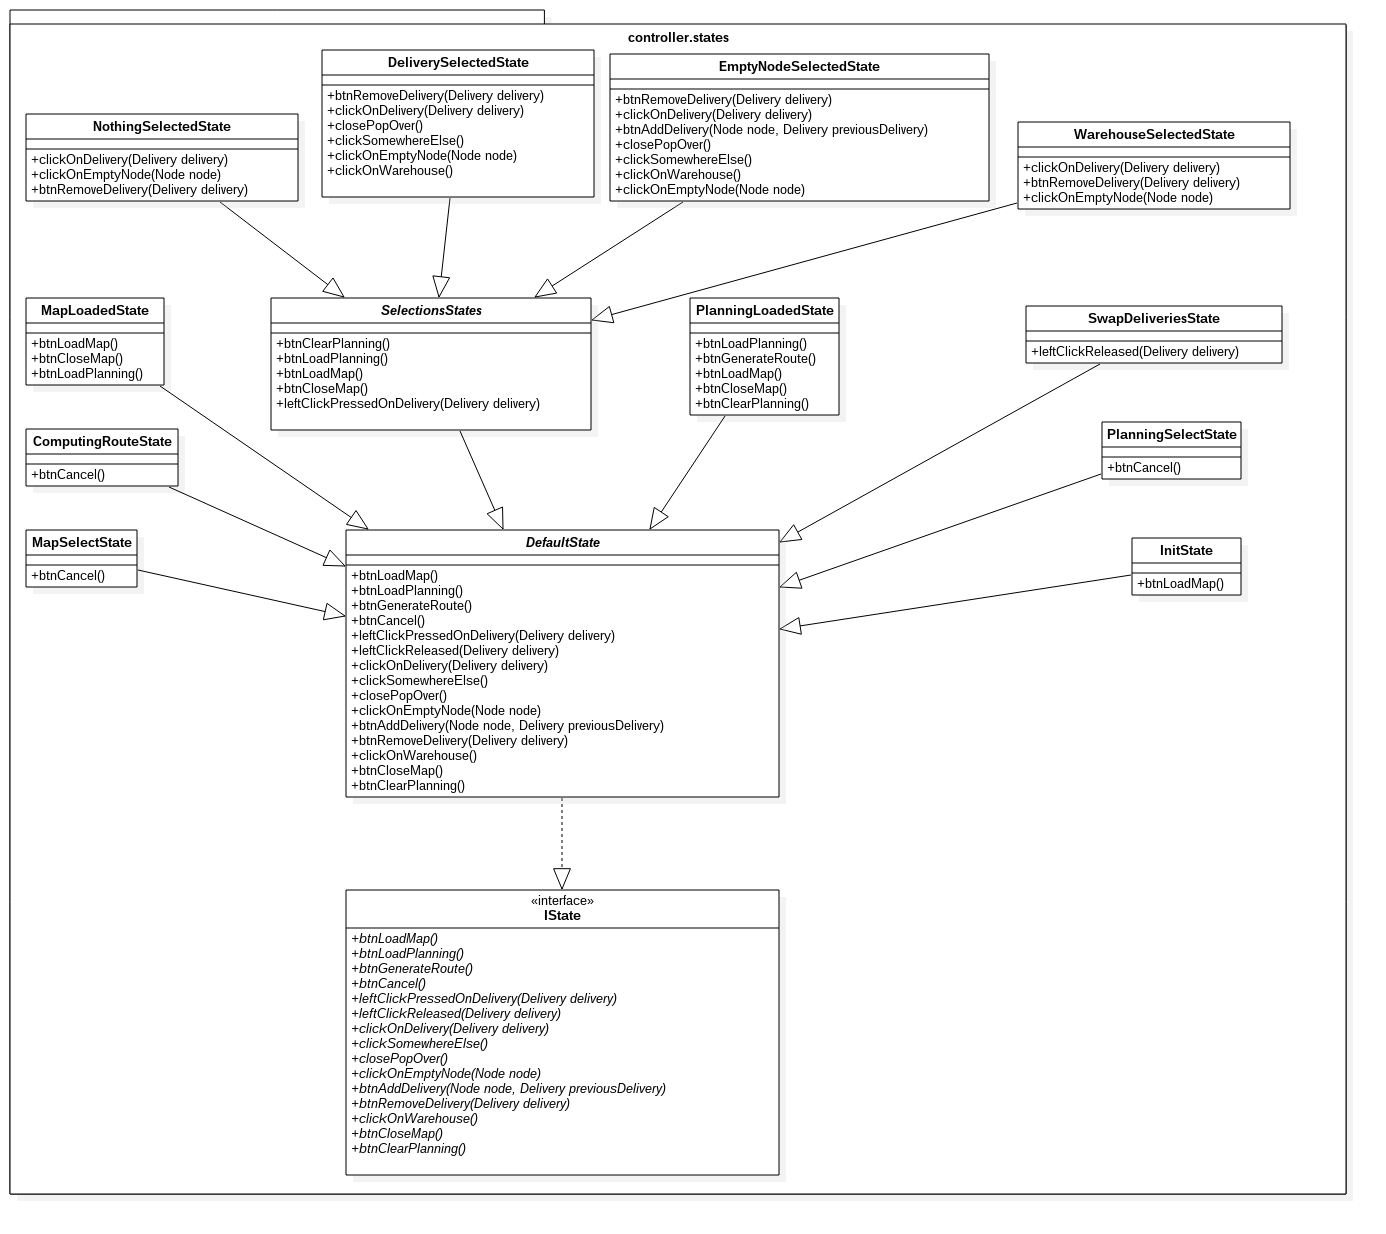
\includegraphics[scale=0.4,angle=0]{figures/controller_states-class.png}}
\caption{Controller States package including classes}
\end{figure}

\begin{figure}[H]
\centering
\noindent\makebox[\textwidth]{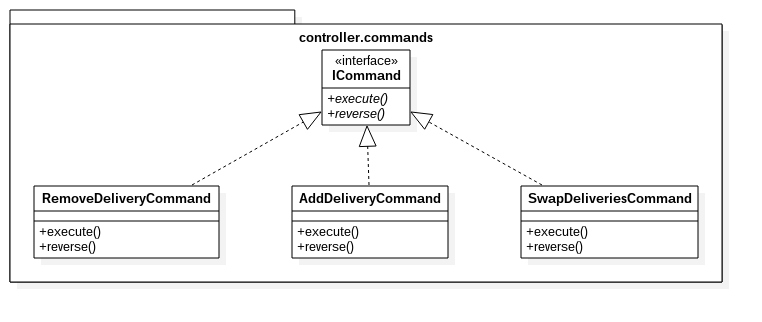
\includegraphics[scale=0.5,angle=0]{figures/controller_commands-class.png}}
\caption{Controller Commands package including classes}
\end{figure}

\subsection{Other diagrams}
\label{subsec:other-diagrams}

The next figure shows utils package which contains all utility classes which can also be called helpers. These objects are used to implement design patterns or - as XML parsers - to provide convenient interfaces to convert data stored in files into objects usable by the application. Further information are available in III.3 section.

\begin{figure}[H]
\centering
\noindent\makebox[\textwidth]{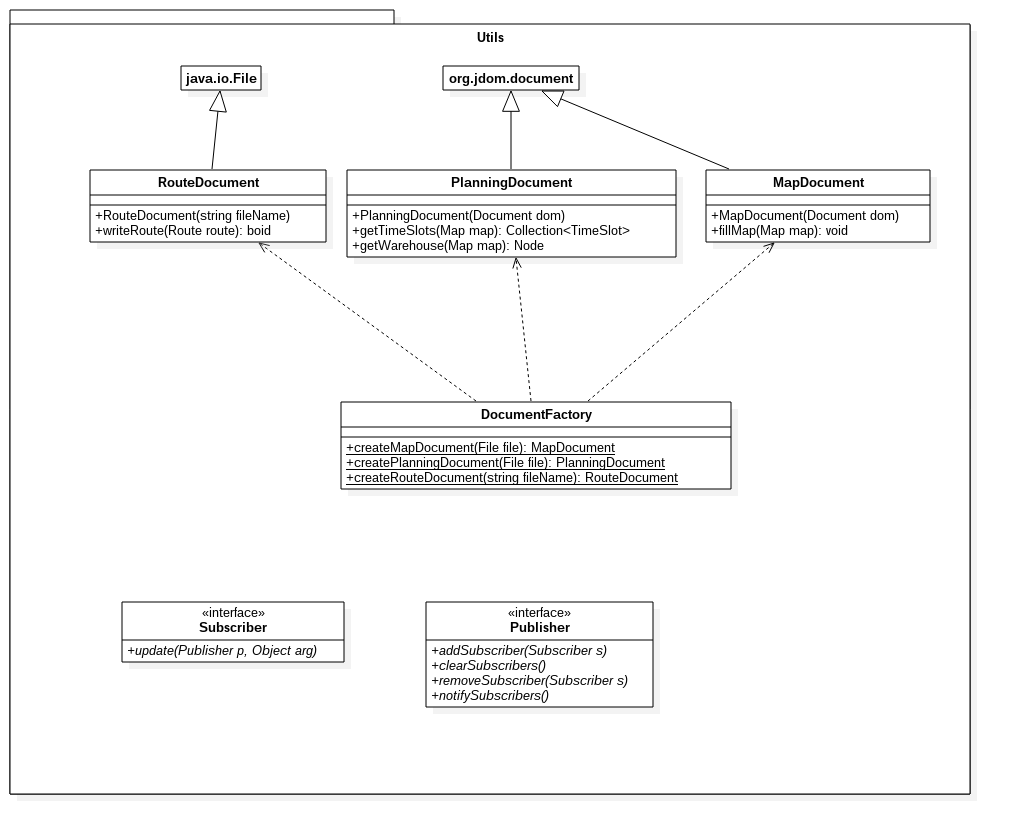
\includegraphics[scale=0.5,angle=0]{figures/utils-class.png}}
\caption{Utils package and its classes}
\end{figure}

\section{Choix architecturaux et patrons de conception utilisés \it{(FR)}}
\label{sec:choix-architecturaux-et-patrons-de-conception-utilises}

\bfit{Les classes citées dans ce document pouvant présenter des ambiguïtés sont référencées dans le glossaire.} \\

Nous choisirons tout d'abord de respecter l'architecture globale de type \bf{MVC} afin de garantir une simplicité de maintenance corrective et évolutive de l'application. Les différents composants appartenant à ces trois grandes catégories (Modèle, Vue et Contrôleur) implémenteront divers patrons de conception. \\

Concernant l'architecture globale, nous avons choisi de faire en sorte que la hiérarchie en couche soit parfaitement respectée, c'est-à-dire que la vue ne modifie en aucun cas le modèle sans  passer par le contrôleur. La vue, cependant, implémente pour certains de ses composants le patron \bf{Observateur} pour détecter les modifications au niveau du modèle et se modifier ou demander au contrôleur d'effectuer des actions en conséquence.\\

Les objets du modèle, qui constituent l'ensemble des données métier manipulées par l'application représentées par des objets, sont pour la plupart des conteneurs de données améliorés et n'implémentent pas de traitements particuliers. Il y a cependant des exceptions, l'objet \bf{Map} implémentant l'algorithme permettant de calculer le plus court chemin entre deux points et l'objet \bf{Planning} permettant de calculer une tournée et de créer l'objet \bf{Route} correspondant. Certains objets, tels que \bf{Map} et \bf{Planning}, constituent en réalité des conteneurs d'autres objets du modèle. Ces objets agissent comme des \bf{Fabrique}s pour les objets qu'ils contiennent. Cela permet de garantir la cohérence des objets contenus dans ces conteneurs ainsi que la maîtrise de la durée de vie de ces derniers. Comme indiqué dans le paragraphe précédent, le modèle est observé par la vue ce qui signifie que certains objets du modèle sont \bf{Observable}s. Il s'agit des objets \bf{Map}, \bf{Planning} et \bf{Route}. Ce mécanisme nous permet de notifier la vue de changements au niveau du modèle. \\

L'objet qui représente la \bf{Map} dans la vue, \bf{MapView}, ainsi que celui qui représente l'arbre des livraisons implémentent le patron \bf{Observateur}. Pour le reste, la vue est isolée du modèle. Celui-ci peut donc fonctionner indépendamment de la vue. \\

Nous avons ajouté un package supplémentaire n'apparaissant pas dans l'architecture MVC afin d'y placer tous les objets étant catégorisés utilitaires. Ces  derniers rendent des services aux autres objets de l'application mais possèdent des traitements qui auraient pu être intégrés aux objets de l'application si nous n'avions pas fait le choix de segmenter les traitements. Ce package, nommé utils, contient notamment des interfaces plus simples pour la création des objets du modèle qui possèdent une représentation sous forme de fichiers XML. Ce package contient également une classe permettant la conversion de types spéciaux propres à l'application et une \bf{Fabrique} pour les objets d'interface avec les fichiers. Nous retrouvons également dans ce package les interfaces et les classes permettant d'utiliser une implémentation générique de l'algorithme de résolution TSP (Traveler Salesman Problem), ce dernier pouvant être utilisé par d'autres modules. \\

Le choix majeur effectué concernant le contrôleur est de séparer les traitements en créant des sous-composants de ce contrôleur principal. Ce package contient donc un ensemble de  contrôleurs spécialisés. Cette organisation au niveau du contrôleur présente de nombreux avantages et notamment la simplification des procédures de gestion des erreurs, leurs causes étant segmentées à l'image des contrôleurs qui peuvent les rencontrer. 
Nous avons donc choisi de dédier un contrôleur à la gestion du modèle, qui constitue en réalité l'interface du contrôleur avec le modèle. Ce contrôleur se nomme \bf{ModelManager} et garantie la cohérence du modèle exploité par l'application, tout en proposant une interface simple pour l'accès au modèle. Il ajoute également un niveau d'encapsulation supplémentaire concernant les données manipulées dans le modèle. 

Un second contrôleur, nommé \bf{IOManager}, est chargé des interactions avec le système de fichiers du système d'exploitation exécutant l'application. C’est à son niveau que sont traitées les erreurs de type Entrée/Sortie telles que l'absence de fichier ou encore les privilèges insuffisants pour lire/écrire un fichier. De nouveau, ce contrôleur propose une interface simple pour effectuer les opérations dont il est chargé. 

Ensuite, l'\bf{UIManager}, est le pendant du \bf{ModelManager}, mais pour l'interface graphique. Il constitue une interface, simple d'utilisation, entre le contrôleur et la vue. Cela permet de centraliser les informations provenant de la vue. C'est aussi le rôle de ce contrôleur d'interpréter les ordres en provenance de la vue pour les convertir en ordres exécutables par le \bf{ContextManager}. 

Le \bf{ContextManager} a deux rôles majeurs qui lui valent d'implémenter deux patrons de conception qui sont le patron \bf{État} et le patron \bf{Commande}. Il a tout d'abord pour rôle d'entretenir la machine à états globale de l'application, c'est-à-dire de garantir à chaque instant qu'une commande utilisateur déclenchera les bons traitements dans l'application et donc les bonnes réactions de l'interface utilisateur et du modèle. Son second rôle est d'entretenir un historique des modifications effectuées de sorte à ce que l'utilisateur puisse défaire et refaire les dernières actions qu'il a effectué. Ce contrôleur assure à l'utilisateur que l'action qu'il veut effectuer a du sens dans le processus global que déroule l'application. Il est dans cette optique étroitement lié à l'\bf{UIManager} qui lui fait parvenir les commandes de l'utilisateur.
Il est, à ce stade, important de préciser que ces différents composants implémentent tous le patron \bf{Singleton} afin de garantir l'unicité de chaque interface et par conséquent l'unicité du modèle, de l'état global de l'application et de l'historique des commandes effectuées.

L'objet \bf{Controller} présent dans le package ne constitue en réalité que le point d'entrée de l'application. Il est appelé par la procédure main qui l'utilise pour initialiser les différents composants du contrôleur, c'est-à-dire réaliser la première instanciation des composants du contrôleur, puis démarrer l'interface graphique.

On peut également considérer l'\bf{UIManager} et le \bf{ModelManager} comme des \bf{Façade}s respectivement pour la vue et le modèle. 

\section{Sequence Diagram describing Route computation process \it{(EN)}}
\label{sec:sequence-diagram-describing-route-computation-process}

\begin{figure}[H]
\centering
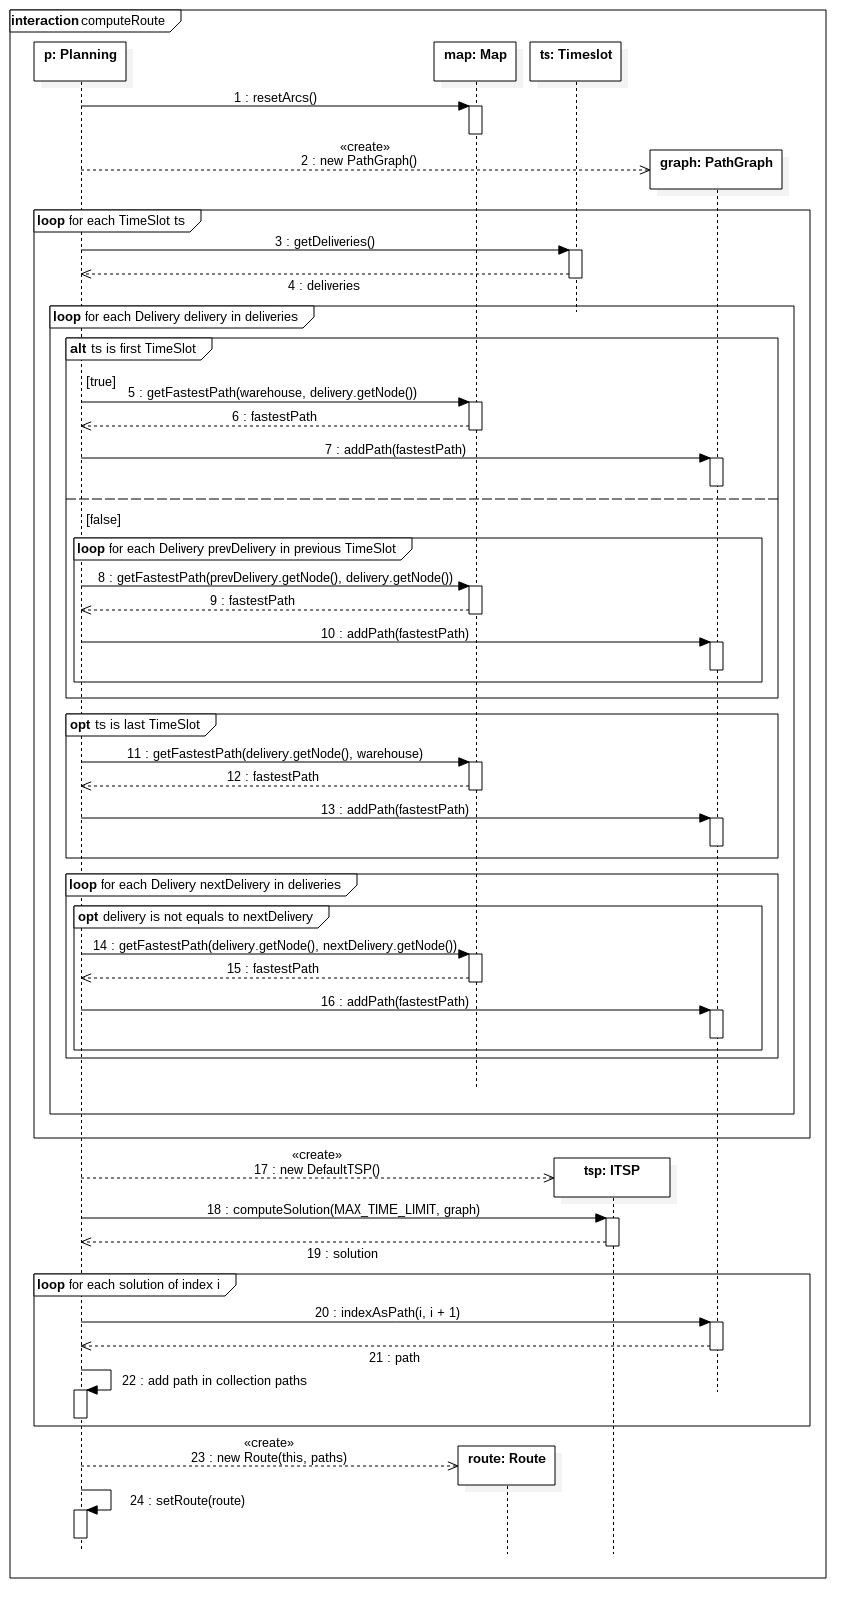
\includegraphics[scale=0.35,angle=0]{figures/sequence-diagram-route-compute.png}
\caption{Sequence diagram describing route computation process}
\end{figure}

The main goal of the application is to figure out what is the best route to deliver in lower times each customer, thanks to a loaded planning. The previous sequence diagram shows us the interactions between the different parts of the model used to compute this route.\\

The \bf{Planning} object is describing all the deliveries’ points, so the method used to start the calculation is \bf{computeRoute}. The main idea of this algorithm, is to build a new graph, that will represent the solutions that could be selected to do the route. In fact, all the deliveries are grouped by time slots. So, in the new graph, the nodes are corresponding to the deliveries - or the warehouse, and the arcs are corresponding to the fastest path between the initial vertex and the terminal vertex. This fastest path is based on the duration time and is computed thanks to a Dijkstra algorithm implementation. This calculation is represented in the sequence diagram by the \bf{getFastestPath(Node startNode, Node endNode)} method, in the \bf{Map} class.\\

So, for each time slot, we find the fastest path between each delivery of the time slot and add the result in the new graph, by calling the \bf{addPath(Path path)} method, in the \bf{PathGraph} class. Then, we do the same between the deliveries of a time slot and the deliveries of the previous time slot, in order to link them. If the current time slot being computed is the first one or the last one, we need to find the fastest path between its deliveries and the warehouse.\\

After we created this new graph, we try to find a solution for doing all the deliveries and come back to the warehouse, by calling the \bf{computeSolution(int maxTimeLimit, IGraph graph)} method, of the \bf{DefaultTSP} class, which implements the Traveler Salesman Problem (TSP) resolution.\\

Then, if the TSP resolution was successful, we can construct the corresponding \bf{Route} object, by getting the correct \bf{Path} objects stored in the \bf{PathGraph} object. The step is done by calling the \bf{indexAsPath(int i, int j)} method. Indeed, the TSP algorithm is done by using numeric indexes to identify the nodes, so we need to convert back the solution’s indexes into real \bf{Path} objects.\\

At this point, the new \bf{Route} is set and can be used by the software.

%%%%%%%%%%%%%%%%%%%%%%%%%%%%%%%%%%%%%%%%%%%%%%% Implémentation et tests

\part{Implémentation et tests}
\label{part:implementation-et-tests}
\setcounter{section}{0}

\section{Notes related to source code and unit tests \it{(EN)}}
\label{sec:notes-related-to-source-code}

\bf{Source code:} After we made the conception and the UML class diagrams, we started to implement them. However, for more efficiency, we chose to use the Java threads and tasks mechanisms, changing a little the implementation but allowing the user to abort long tasks and do not block the user interface.\\

\bf{Unit tests:} All the tests have been realized thanks to JUnit, a unit-testing framework for Java. We have done the tests of all the classes of the model, and also the test of the utility classes (utils package). The principle of this framework is simply to test if the expected result of the tested method is the same as the resultat we really get from this method. The testing method of JUnit looks like that : \it{assertEquals(expectedResult, actualResult)}. If the two objects are not equals, an AssertionError is thrown. We have tried to test as much cases as possible, so sometimes a method can have more than one \it{assertEquals} test.
 
\section{Packages and classes diagrams generated from source code \it{(EN)}}
\label{sec:packages-and-classes-diagrams-generated-from-source-code}

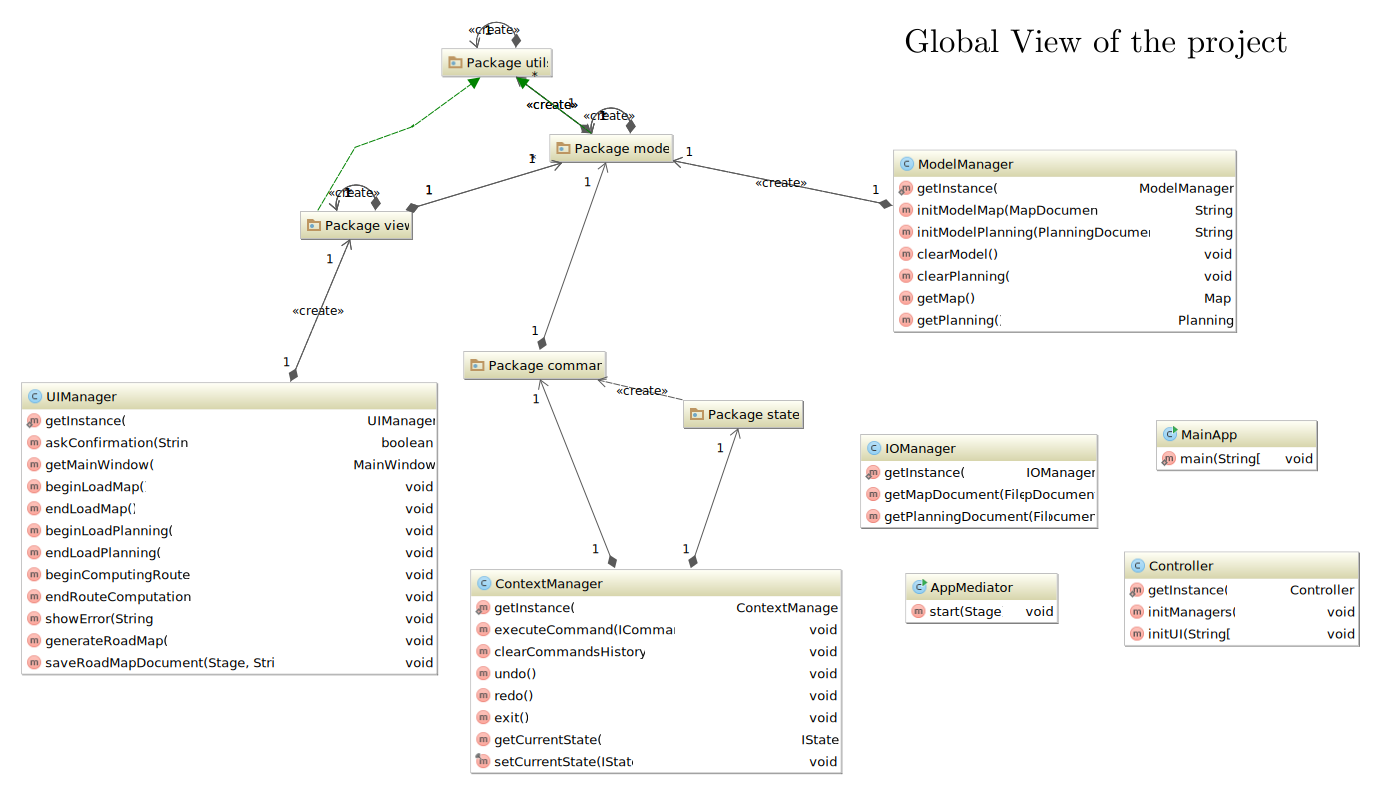
\includepdf{figures/package}
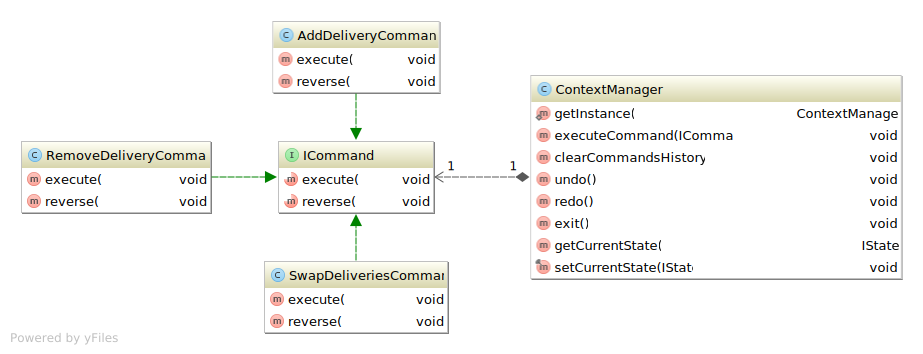
\includepdf{figures/command}
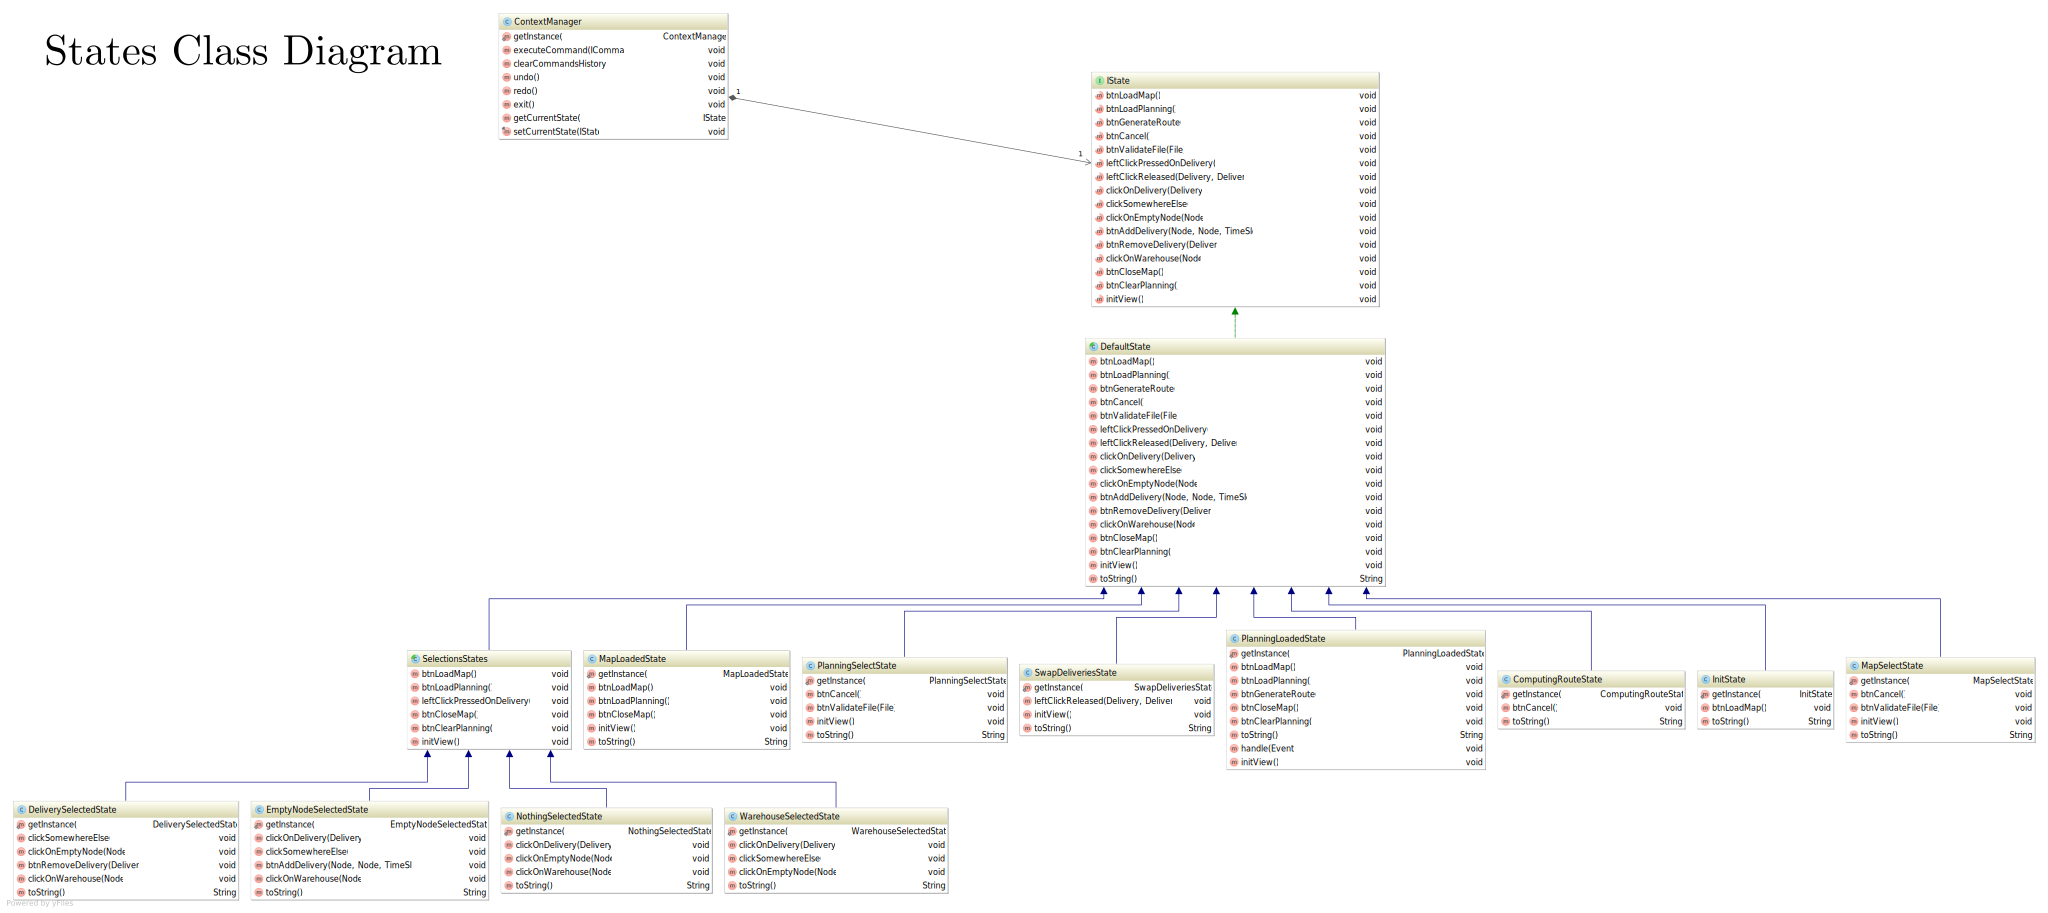
\includepdf{figures/states}
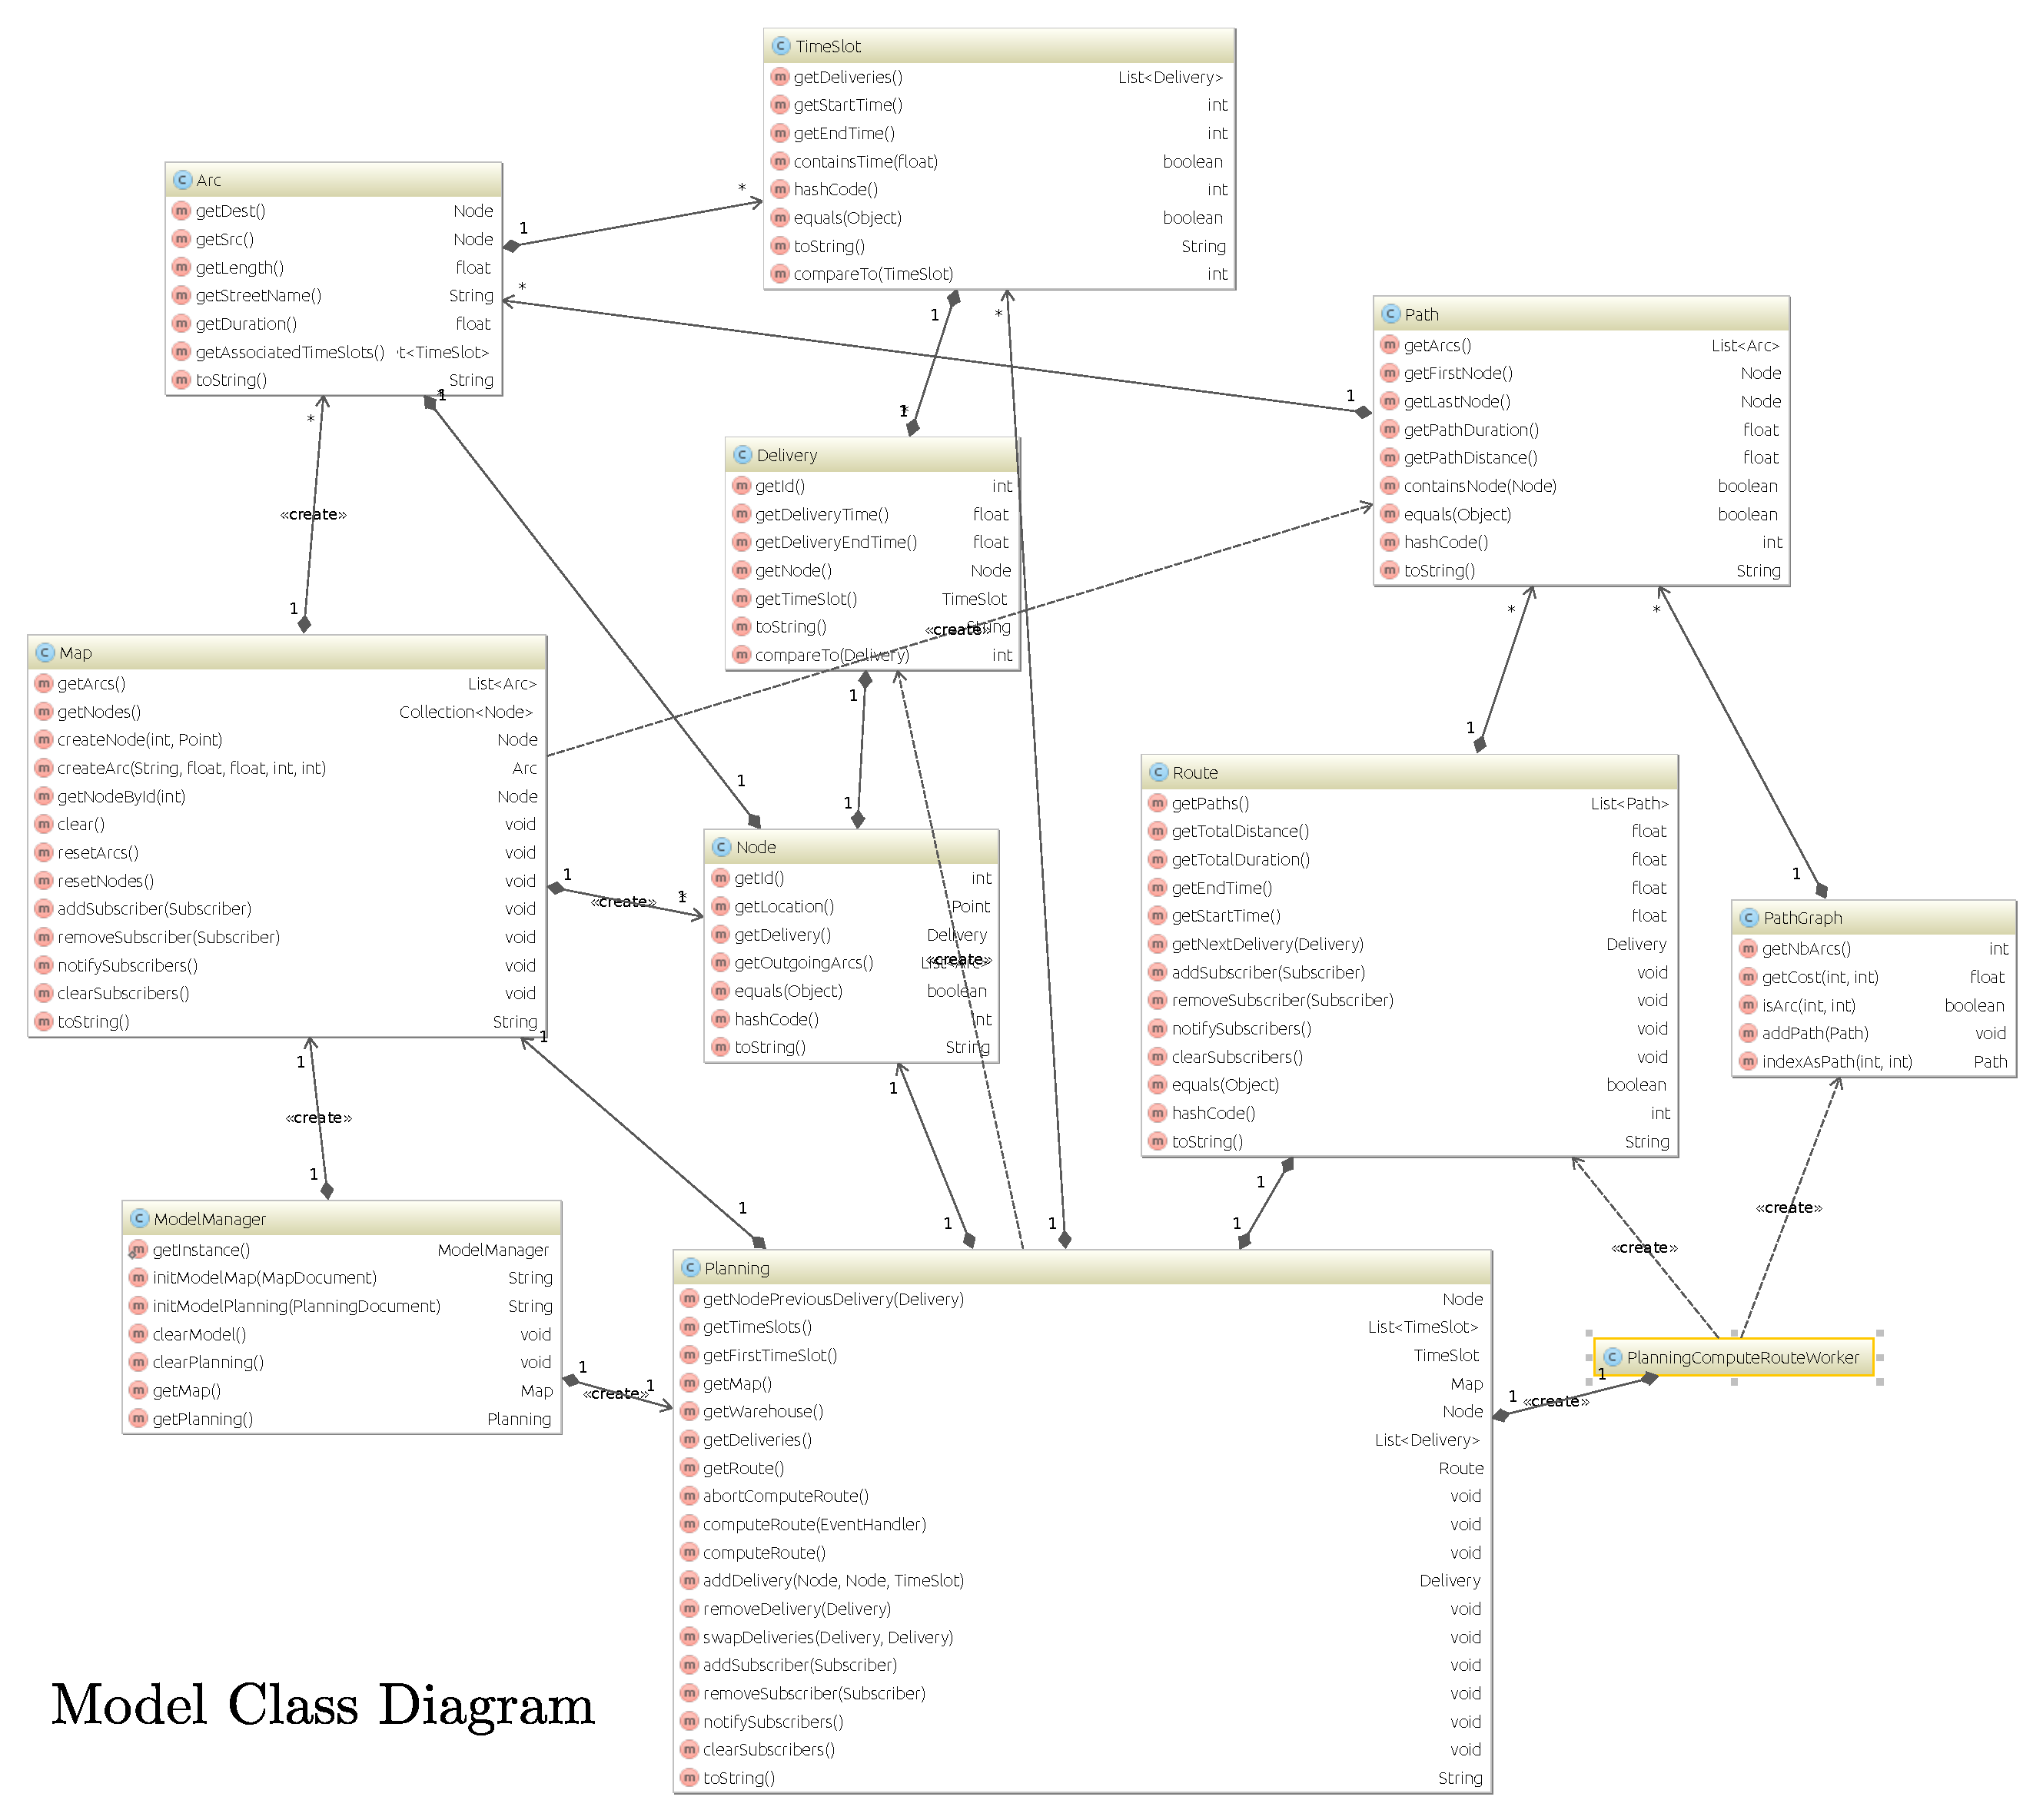
\includepdf{figures/model}
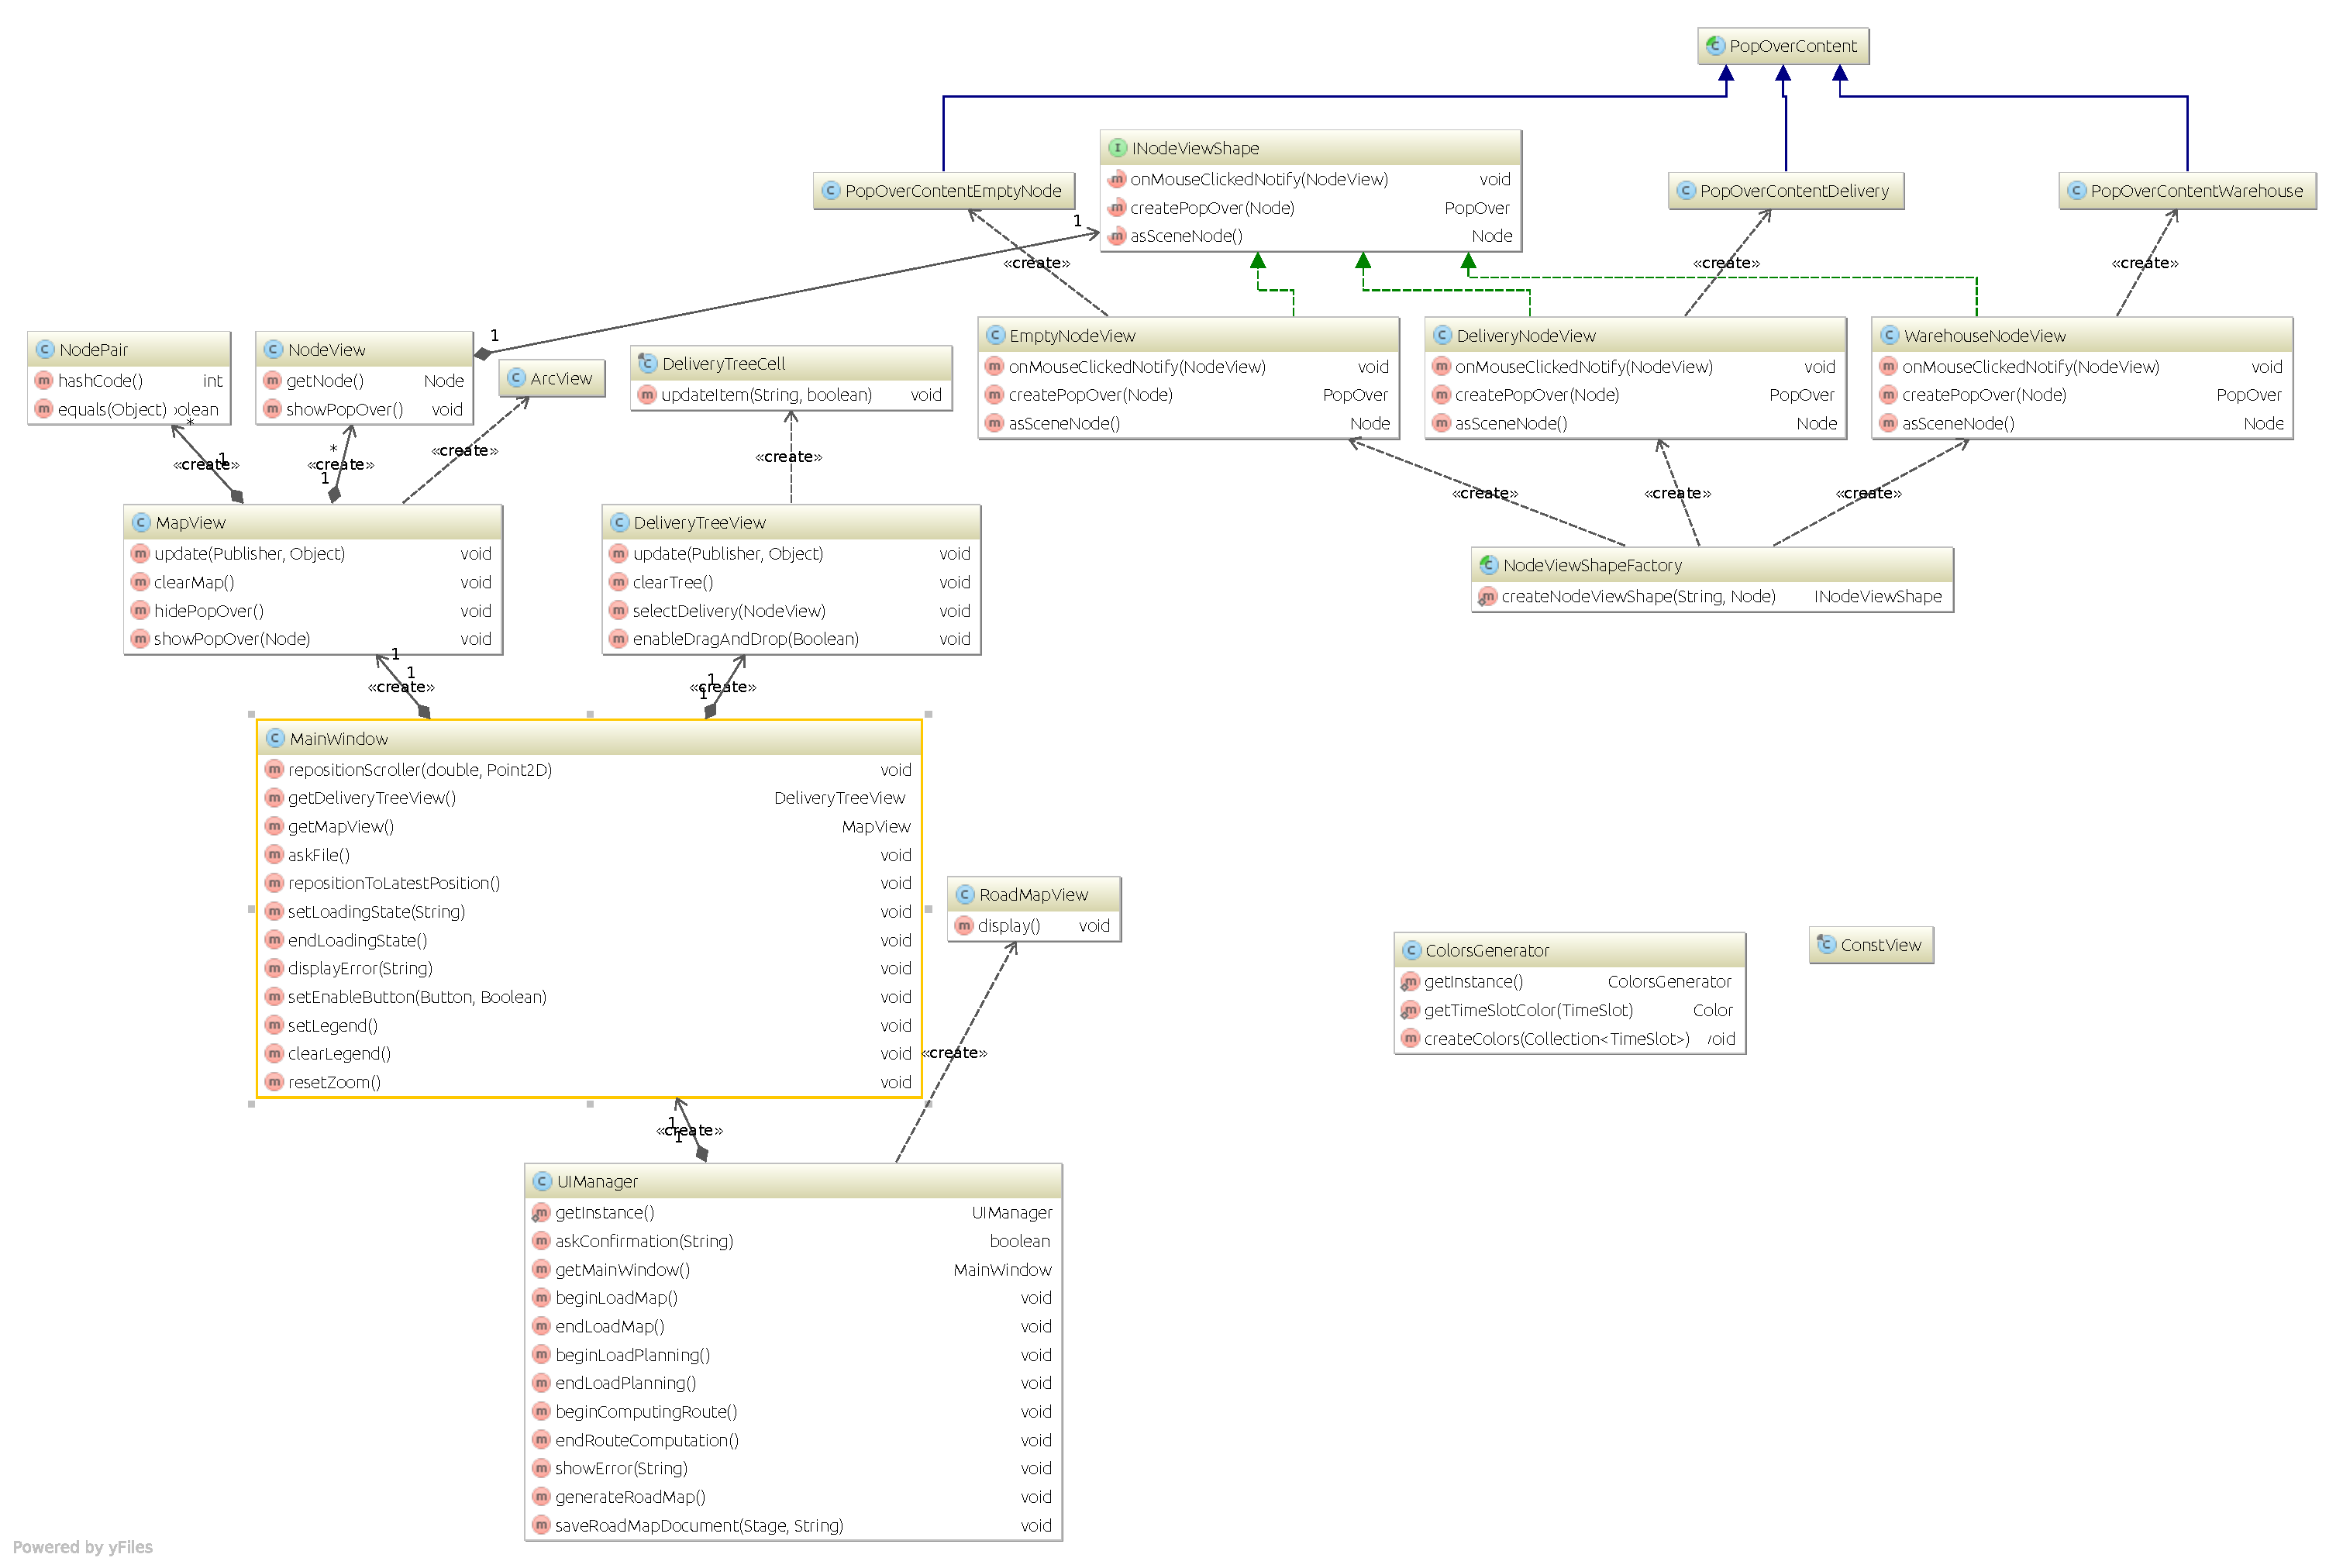
\includepdf{figures/view}

%%%%%%%%%%%%%%%%%%%%%%%%%%%%%%%%%%%%%%%%%%%%%%%%%%%%%%%%%%%%%%%% Bilan

\part{Bilan}
\label{part:bilan}
\setcounter{section}{0}

\section{Planning effectif du projet \it{(FR)}}
\label{sec:planning-effectif-du-projet}

Voici le planning effectif du projet sous forme d'un Gantt. Comme vous pouvez le voir il diffère du prévisionnel avec un grand nombre de tâche supplémentaire et un redécoupage en sous-tâche.

\begin{figure}[H]
\centering
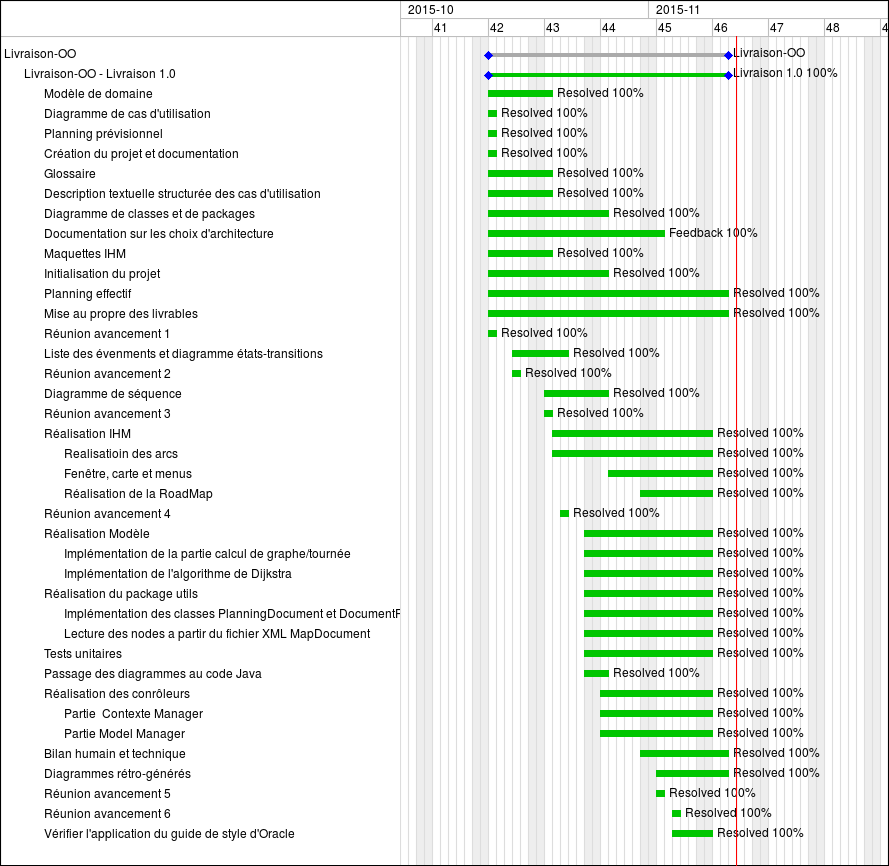
\includegraphics[scale=0.5,angle=0]{redmine/gantt-real.png}
\caption{Planning effectif}
\end{figure}

\section{Temps passés sur les tâches \it{(FR)}}
\label{sec:temps-passes-sur-les-taches}

Le suivi de projet a été fait en utilisant l'outil Redmine. Vous trouverez en annexe (cf. \ref{sec:cr-des-taches-redmine}~Compte-rendu des tâches) un aperçu des temps assignés et des temps passés pour chaque tâche. L'affectation correspond à la personne en charge de cette tâche, mais cela ne veut pas dire que les autres membres de l'hexanôme n'ont pas travaillé dessus.

Voici le détail des heures effectuées par chaque personne :

\begin{figure}[H]
\centering
\pgfplotstabletypeset[
    col sep=semicolon,
    string type,
    columns={Utilisateur,Temps total},
    columns/Utilisateur/.style={column name=Utilisateur, column type={|l}},
    columns/Temps total/.style={column name=Temps Total (heures), column type={|r|}},
    every head row/.style={before row=\hline,after row=\hline},
    every last row/.style={before row=\hline,after row=\hline},
    ]{redmine/users-time.csv}
\caption{Temps passés par personne}
\end{figure}

Vous trouverez en annexe le détail par demande des temps passés (cf. \ref{sec:details-des-temps-passes}~Détail des temps passés) ainsi que le détail par tâche (cf. \ref{sec:cr-des-taches-redmine}~Compte-rendu des tâches).

\section{Bilan humain et technique \it{(FR)}}
\label{sec:bilan-humain-et-technique}

\subsection{Dépassements des estimations}
\label{subsec:depassements-des-estimations}

Comme présenté dans le planning effectif et les temps passés, nous avons fait un dépassement sur plusieurs estimations. Tout d'abord, il faut prendre en compte que nous avions peu d'expérience pour estimer ce projet et c'est une qualité qui s'obtient avec l’entraînement et l'expérience.

Nous avons fait le choix d'utiliser l'outil JavaFX afin d'acquérir de nouvelles compétences. L'apprentissage a pris beaucoup plus de temps de prévu ce qui explique le dépassement sur l'implémentation de l'IHM. De plus, nous avions fait le choix de lancer en autonomie un membre de l'équipe, le rendant indispensable pour toute modification sur la partie vue de notre programme. Cela a provoqué un ralentissement global pour l'assemblage des trois composantes (contrôleur, vue et modèle).

Nous pouvons aussi noter un dépassement sur la partie conception. C'est l'une des tâches les plus importantes et nous avons préféré passer plus de temps sur ce point avant de commencer l'implémentation pour éviter des dépassements plus importants par la suite (notamment sur la partie modèle). Cependant, un manque de focalisation sur cette étape conceptuelle peut également expliquer ces dépassements d'horaires. En effet, l'envie d'avoir rapidement un rendu visuel et fonctionnel a tendance à détourner les développeurs de cette tâche. Des recentrages ont notamment été nécessaires sur les parties vue et contrôleur, afin de terminer en premier lieu cette étape de conception.

Même si les tâches de gestion de projet, d'analyse et de bilan sont plutôt correctes, le chiffrage général reste bien trop bas par rapport au réel et il est important de le noter pour les projets futurs.

\subsection{Bilan humain et ressentis des membres}
\label{subsec:bilan-humain}

Globalement le projet c'est bien passé. Nous sommes arrivés à termes du projet et nous avons réussi à implémenter tous les scénarios prévus lors du lancement du projet. Cependant, nous avons eu quelques points négatifs sur le plan humain.

Ce projet était notre première occasion de réaliser un projet en grande équipe (7 membres), tout en devant réaliser les différentes phases d'un projet, de l'analyse jusqu'à l'implémentation. Il apparaît que sur des projets de plus petite taille, les écarts de niveau est bien moins visible, tandis qu'ici, chaque membre a son importance et le ralentissement de l'un d'eux provoque un retard global sur le projet. Les différentes expériences en entreprise chez les uns et les autres amplifient également ce phénomène.

Un ressenti partagé par l'ensemble de l'équipe a été qu'il n'ait pas été possible de toucher à tout et intervenir dans n'importe quelle partie du projet. Ce changement est spécifiquement dû au fait que chaque personne se spécialise dans le rôle qu'on lui a donné et qu'on ne peut pas se permettre de passer plusieurs heures supplémentaires à comprendre l'ensemble des mécanismes mis en place par les autres. Notamment, nous avons remarqué des spécialisations pour JavaFX, pour le calcul de la tournée, pour la gestion des fichiers XML ou encore une autre pour le fonctionnement de la machine à état.

Cependant, nous pouvons relever comme points positifs, que techniquement nous avons bien progressé. La mise en pratique des designs patterns nous a permis d’acquérir de nouvelles visions sur la conception et a engendré un meilleur projet sur le point de vue maintenance et durabilité.

Enfin, nous avons réussi à garder notre calme et une certaine bonne ambiance dans l'équipe malgré des périodes de travail intense ou de pression en raison de la charge de travail plus conséquente en cette période. Nous avons donc tout de même pu rester productif et gagner en efficacité, tout en augmentant la cohésion de groupe et en devenant plus soudés.

\subsection{Bilan technique}
\label{subsec:bilan-technique}

Nous avons eu la possibilité de réaliser ce projet en Java ou en C++. Le niveau technique de notre hexanôme favorisant davantage le Java, nous avons naturellement choisi cette solution technique. Cependant, nous avons décidé de profiter de ce projet pour acquérir tout de même de nouvelles compétences techniques, en plus de celles visées initialement par le cadre du projet.\\

Tous les membres de notre hexanôme connaissant Swing, nous avons effectué le choix de nous tourner vers JavaFX, malgré notre ignorance à ce sujet. Cela nous a permis d'apprendre cette nouvelle technologie, qui est maintenant favorisée par Java 8. \\

Nous avons également profité de ce projet pour mettre en application nos connaissances sur Java, notamment en ajoutant une gestion de tâches multi-thread, nous permettant ainsi d'implémenter des traitements sans pour autant bloquer la vue graphique. En effet, ce projet pouvant proposer des temps de traitement assez longs (beaucoup de points de livraison à traiter par exemple), nous nous sommes confrontés au questionnement de l'expérience utilisateur et de l'ergonomie de notre application. Cette mise en place multi-thread nous a ainsi permis de proposer à l'utilisateur d'interrompre les-dites actions pouvant durer longtemps.\\

Ainsi, ce projet a été l'occasion pour nous de découvrir principalement JavaFX, tout en s'initiant aux questions ergonomiques.

\subsection{Synthèse}
\label{subsec:synthese}

Pour synthétiser, c'est un très bon projet, techniquement comme humainement. Nous avons eu la chance de mettre en pratique du savoir théorique comme l'enseignement des designs patterns mais aussi l’expérience de chacun au travers des différents stages.


%%%%%%%%%%%%%%%%%%%%%%%%%%%%%%%%%%%%%%%%%%%%%%%%%%%%%%%%%%%%%%%% Annexes

\part{Annexes}
\label{part:annexes}
\setcounter{section}{0}

\section{Errors lists \it{(EN)}}
\label{sec:errors-lists}


\subsection{IO Errors List}
\label{subsec:io-errors-list}

This section presents a list of errors which can occur during Input/Output operations such as reading or writing files. \\

\textbf{Input errors :}
\begin{itemize}
  \item[•] \textbf{Cant Read File Error :} the folder is not readable, user’s privileges doesn’t match required privileges.
  \item[•] \textbf{Missing File Error :} the file is missing in the OS File System. \\
\end{itemize}

\textbf{Output errors :}
\begin{itemize}
  \item[•] Cant Write File Error : the folder is not writable, user’s privileges don’t match required privileges.  
\end{itemize}

\subsection{XML errors list}
\label{subsec:xml-errors-lists}

The following lists presents all errors which can be found when reading input XML files.\\

This list contains errors shared by both map definition file and planning definition file.\\

\textbf{Shared errors:}
\begin{itemize}
  \item[•] \textbf{Syntax errors :}
  \begin{itemize}
    \item[•] \textbf{Unexpected End Of File Error :} XML file is not well formatted, tags are not closed properly.\\
  \end{itemize}
\end{itemize}

The next list contains all semantic errors that can occur when parsing XML data. Errors are sorted by file.\\ 

\textbf{File specific errors :}
\begin{itemize}
  \item[•] \textbf{Semantic errors :}
  \begin{itemize}
    \item[•] \textbf{Map file :}
    \begin{itemize}
      \item[•] \textbf{Empty Map Error :} root tag has no child.
      \item[•] \textbf{Missing Node Attribute :} missing id, x or y attribute.
      \item[•] \textbf{Empty Node Error :} tag Node has no outgoing arc.
      \item[•] \textbf{Duplicate Node ID Error :} two or more nodes share the same ID.
      \item[•] \textbf{Duplicate Node Error :} two or more nodes share the same coordinates.
      \item[•] \textbf{Duplicate Arc Error :} two or more outgoing arcs of a single node share the same destination node. 
      \item[•] \textbf{Missing Destination Node Error :} the node referenced by an arc as its destination doesn’t exist. 
      \item[•] \textbf{Invalid Average Speed Value Error :} an arc specified average speed is missing, negative or zero. 
      \item[•] \textbf{Invalid Length Value Error :} an arc specified length is missing, negative or zero.
    \end{itemize}

    \item[•] \textbf{Planning file :}
    \begin{itemize}
      \item[•] \textbf{Missing Warehouse Error :} warehouse tag is missing or the id of the specified warehouse doesn’t match any of the node in the Map.
      \item[•] \textbf{Duplicate Warehouse Error :} more than one warehouse tag is present in the input file.
      \item[•] \textbf{Missing TimeSlot Error :} the file doesn’t specify a timeslot.
      \item[•] \textbf{Duplicate TimeSlot Error :} two or more timeslots have the same start time and end time.
      \item[•] \textbf{Null TimeSlot Error :} a timeslot has the same start and end time.
      \item[•] \textbf{Intersecting TimeSlot Error :} two or more timeslots are intersecting.
      \item[•] \textbf{Reversed TimeSlot Error :} at least one timeslot has its startTime greater than its endTime.
      \item[•] \textbf{Missing Delivery Node Error :} the address specified by a delivery doesn’t match any node in the Map.
      \item[•] \textbf{Duplicate Delivery Error :} two or more deliveries share the same destination. 
    \end{itemize}
  \end{itemize}
\end{itemize}

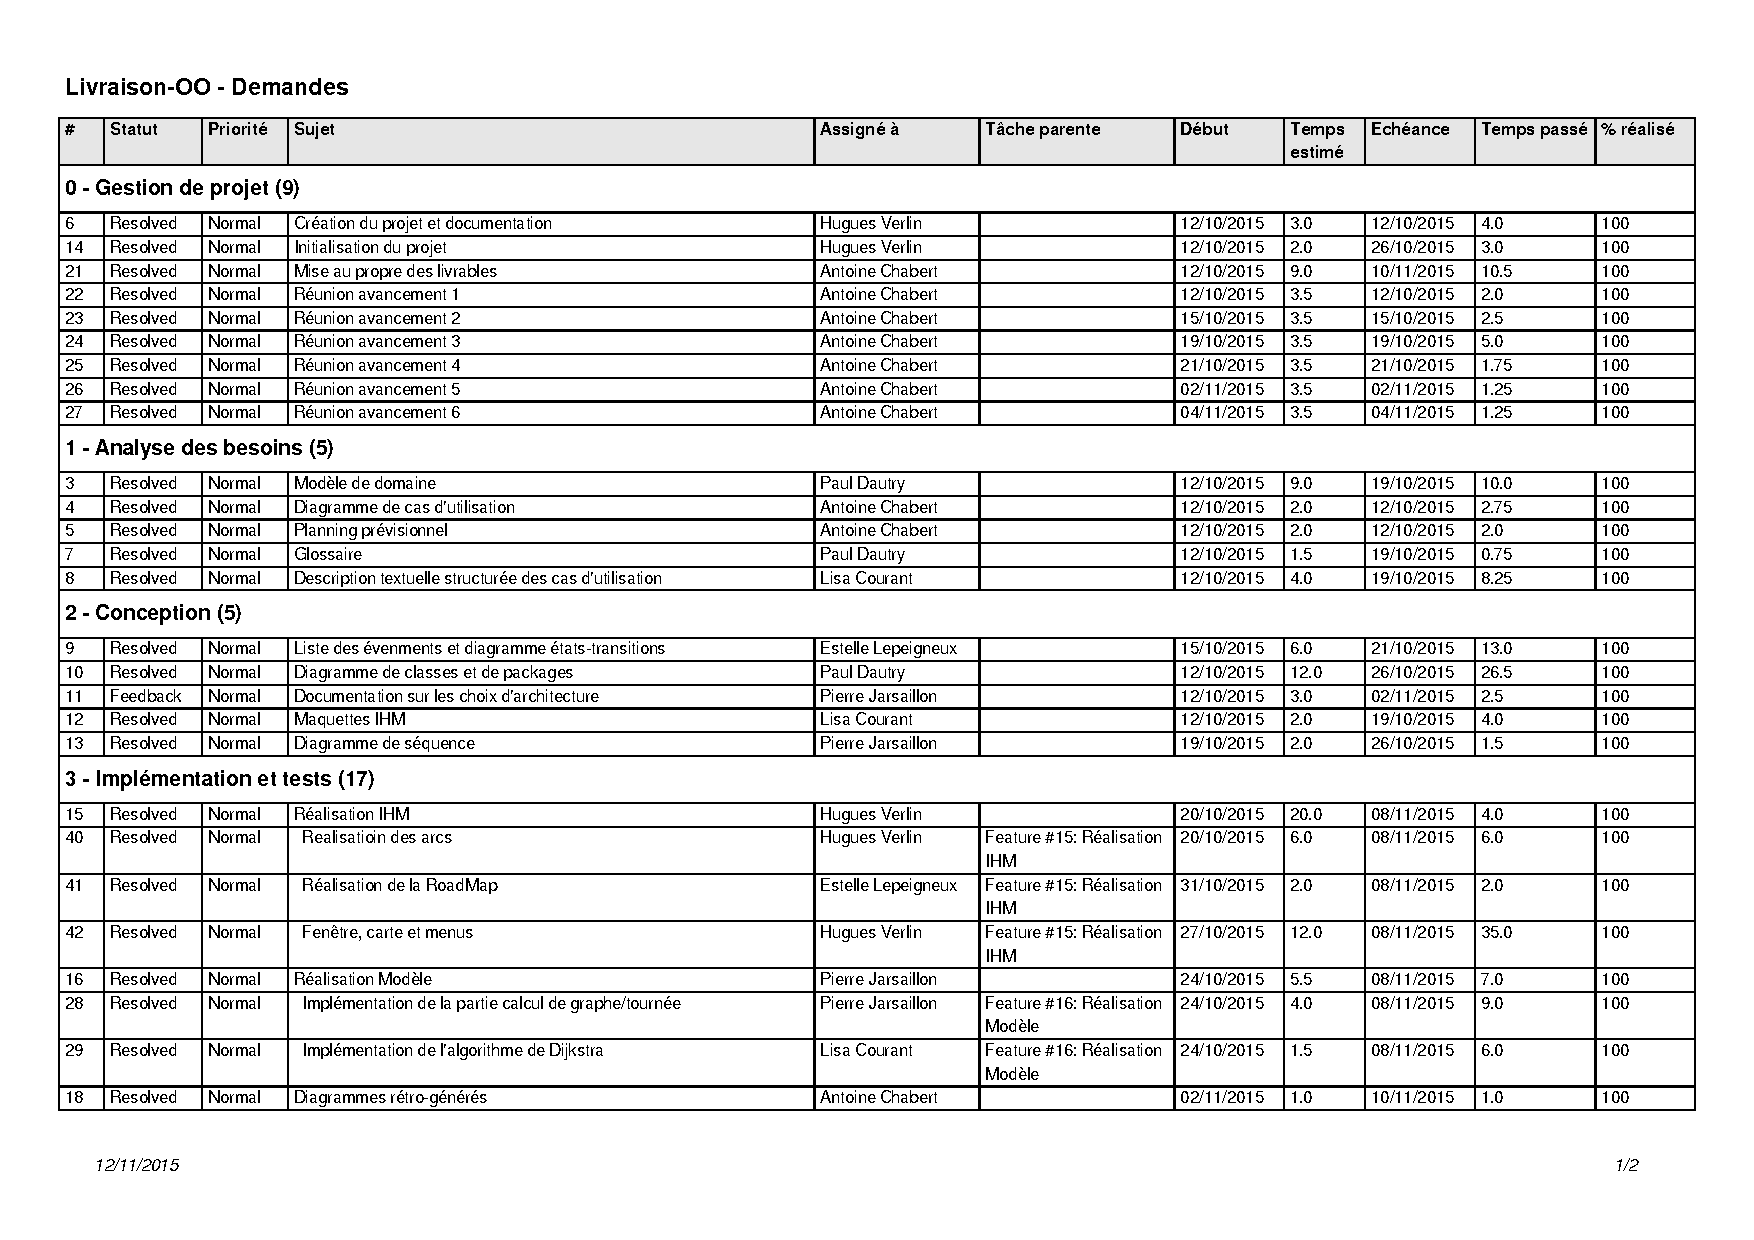
\includepdf[scale=0.8,angle=90,pages={1},pagecommand=\section{Compte-rendu des tâches - Page 1}]{redmine/list-issues-redmine.pdf}
\label{sec:cr-des-taches-redmine}
\includepdf[scale=0.8,angle=90,pages={2},pagecommand=\section{Compte-rendu des tâches - Page 2}]{redmine/list-issues-redmine.pdf}

\section{Détails des temps passés}
\label{sec:details-des-temps-passes}

\begin{figure}[H]
\centering
\noindent\scalebox{0.6}{\pgfplotstabletypeset[
    col sep=semicolon,
    string type,
    columns={Utilisateur,Demande,Temps total},
    columns/Utilisateur/.style={column name=Utilisateur, column type={|l}},
    columns/Demande/.style={column name=Demande, column type={|l}},
    columns/2015/.style={column name=2015, column type={|l}},
    columns/Temps total/.style={column name=Temps Total (heures), column type={|r|}},
    every head row/.style={before row=\hline,after row=\hline},
    every last row/.style={before row=\hline,after row=\hline},
    ]{redmine/users-time-by-issue.csv}}
\caption{Temps passés par personne}
\end{figure}

%%% End document
\end{document}
